% Intro section
	% Describe deviations from plan including difficulties which were encountered
	% Describe the operation of the application with pseudocode
	% Present a critical evaluation of the application
This chapter will cover how the project was created and evaluated. It will begin by describing any deviations from the planned development process including any problems which were encountered and how they were addressed. It will then continue to describe how the final version of the application operates with a pseudocode description. Finally it will present the previously outlined critical evaluation covering validation, reliability, alternative comparison, and professional opinion.
\subsection{Deviation from Plan}
	\subsubsection{Development Approach}
		% Organic dev approach
		% Didn't know what processes the app would use
		As described in section \ref{sec:project_management} it was unsure which approach would be undertaken during the development stages of the project. Once the development stage was reached, an organic approach was taken. Although less structured than an agile methodology it was concluded that removal of the sprint process would allow development of the application to progress quicker as items would not need to be delayed for the next sprint cycle. Allowing problems to be addressed immediately proved useful as the application was not left in an unusable state while other features were produced.
		\\\\
		The log produced by the development stage can be seen in appendix \ref{app:dev_log}. This shows that suitable work was carried out within the time-frame allocated despite using a less structured process and the application includes suitable functionality to complete its aims.
	\subsubsection{Use of EXIF Data and Reference Point}
		Mentioned in section \ref{sec:taking_measurements}, the process which the application would use to produce measurements was undecided and required experimentation. Initially utilising \gls{exif} data from the image was used; this was successful until collection of the sensor size was required. Due to this being uncommon in \gls{exif} data, particularly in images taken with smartphone cameras, this method was dropped for utilisation of a reference point. The code produced during this experimentation period can be seen in appendix \ref{app:exif_code}, the function {\ttfamily get\_sensor\_size} is incomplete as this is where the process was dropped.
		\\\\
		The reference point chosen is a red circular sticker as these are cheap and easy to find in stores or online and a circle was selected over a square or other shape as the orientation of the object does not need to be taken into account. This sticker is applied to the shock so it can be picked up from the image by its colour; locating the reference point was simple though the measuring process produced issues which will be discussed in a following section.
	\subsubsection{Colour Quantification}
		For initial experimentation with using a reference point, the red circle was added to images manually using an image processing application. This allowed for tuning of the colour masking process and to develop the process before using a real reference point on the shock.
		\\\\
		When images with a real reference point were used, the application could not find it. Because the colour range for the masking process was using perfect red (RGB 255,0,0) the non-uniform reds of the sticker in the image were not within this range. These boundaries were expanded to suit the range in the image though this was not enough.
		\\\\
		To solve this issue a further image processing technique was implemented known as colour quantification which reduces an image to 2, 4, 8, 16, or 32 bit colour spaces. By reducing the range of colours in an image detail is lost and objects become more apparent. The difference between an original image and quantified colours is shown in figure \ref{fig:quantified_colours}. Quantifying the colours to 8 bit makes the reference point a flat tone of red while maintaining its shape allowing for the masking process to function correctly.
		\begin{figure}[h!]
			\centering
			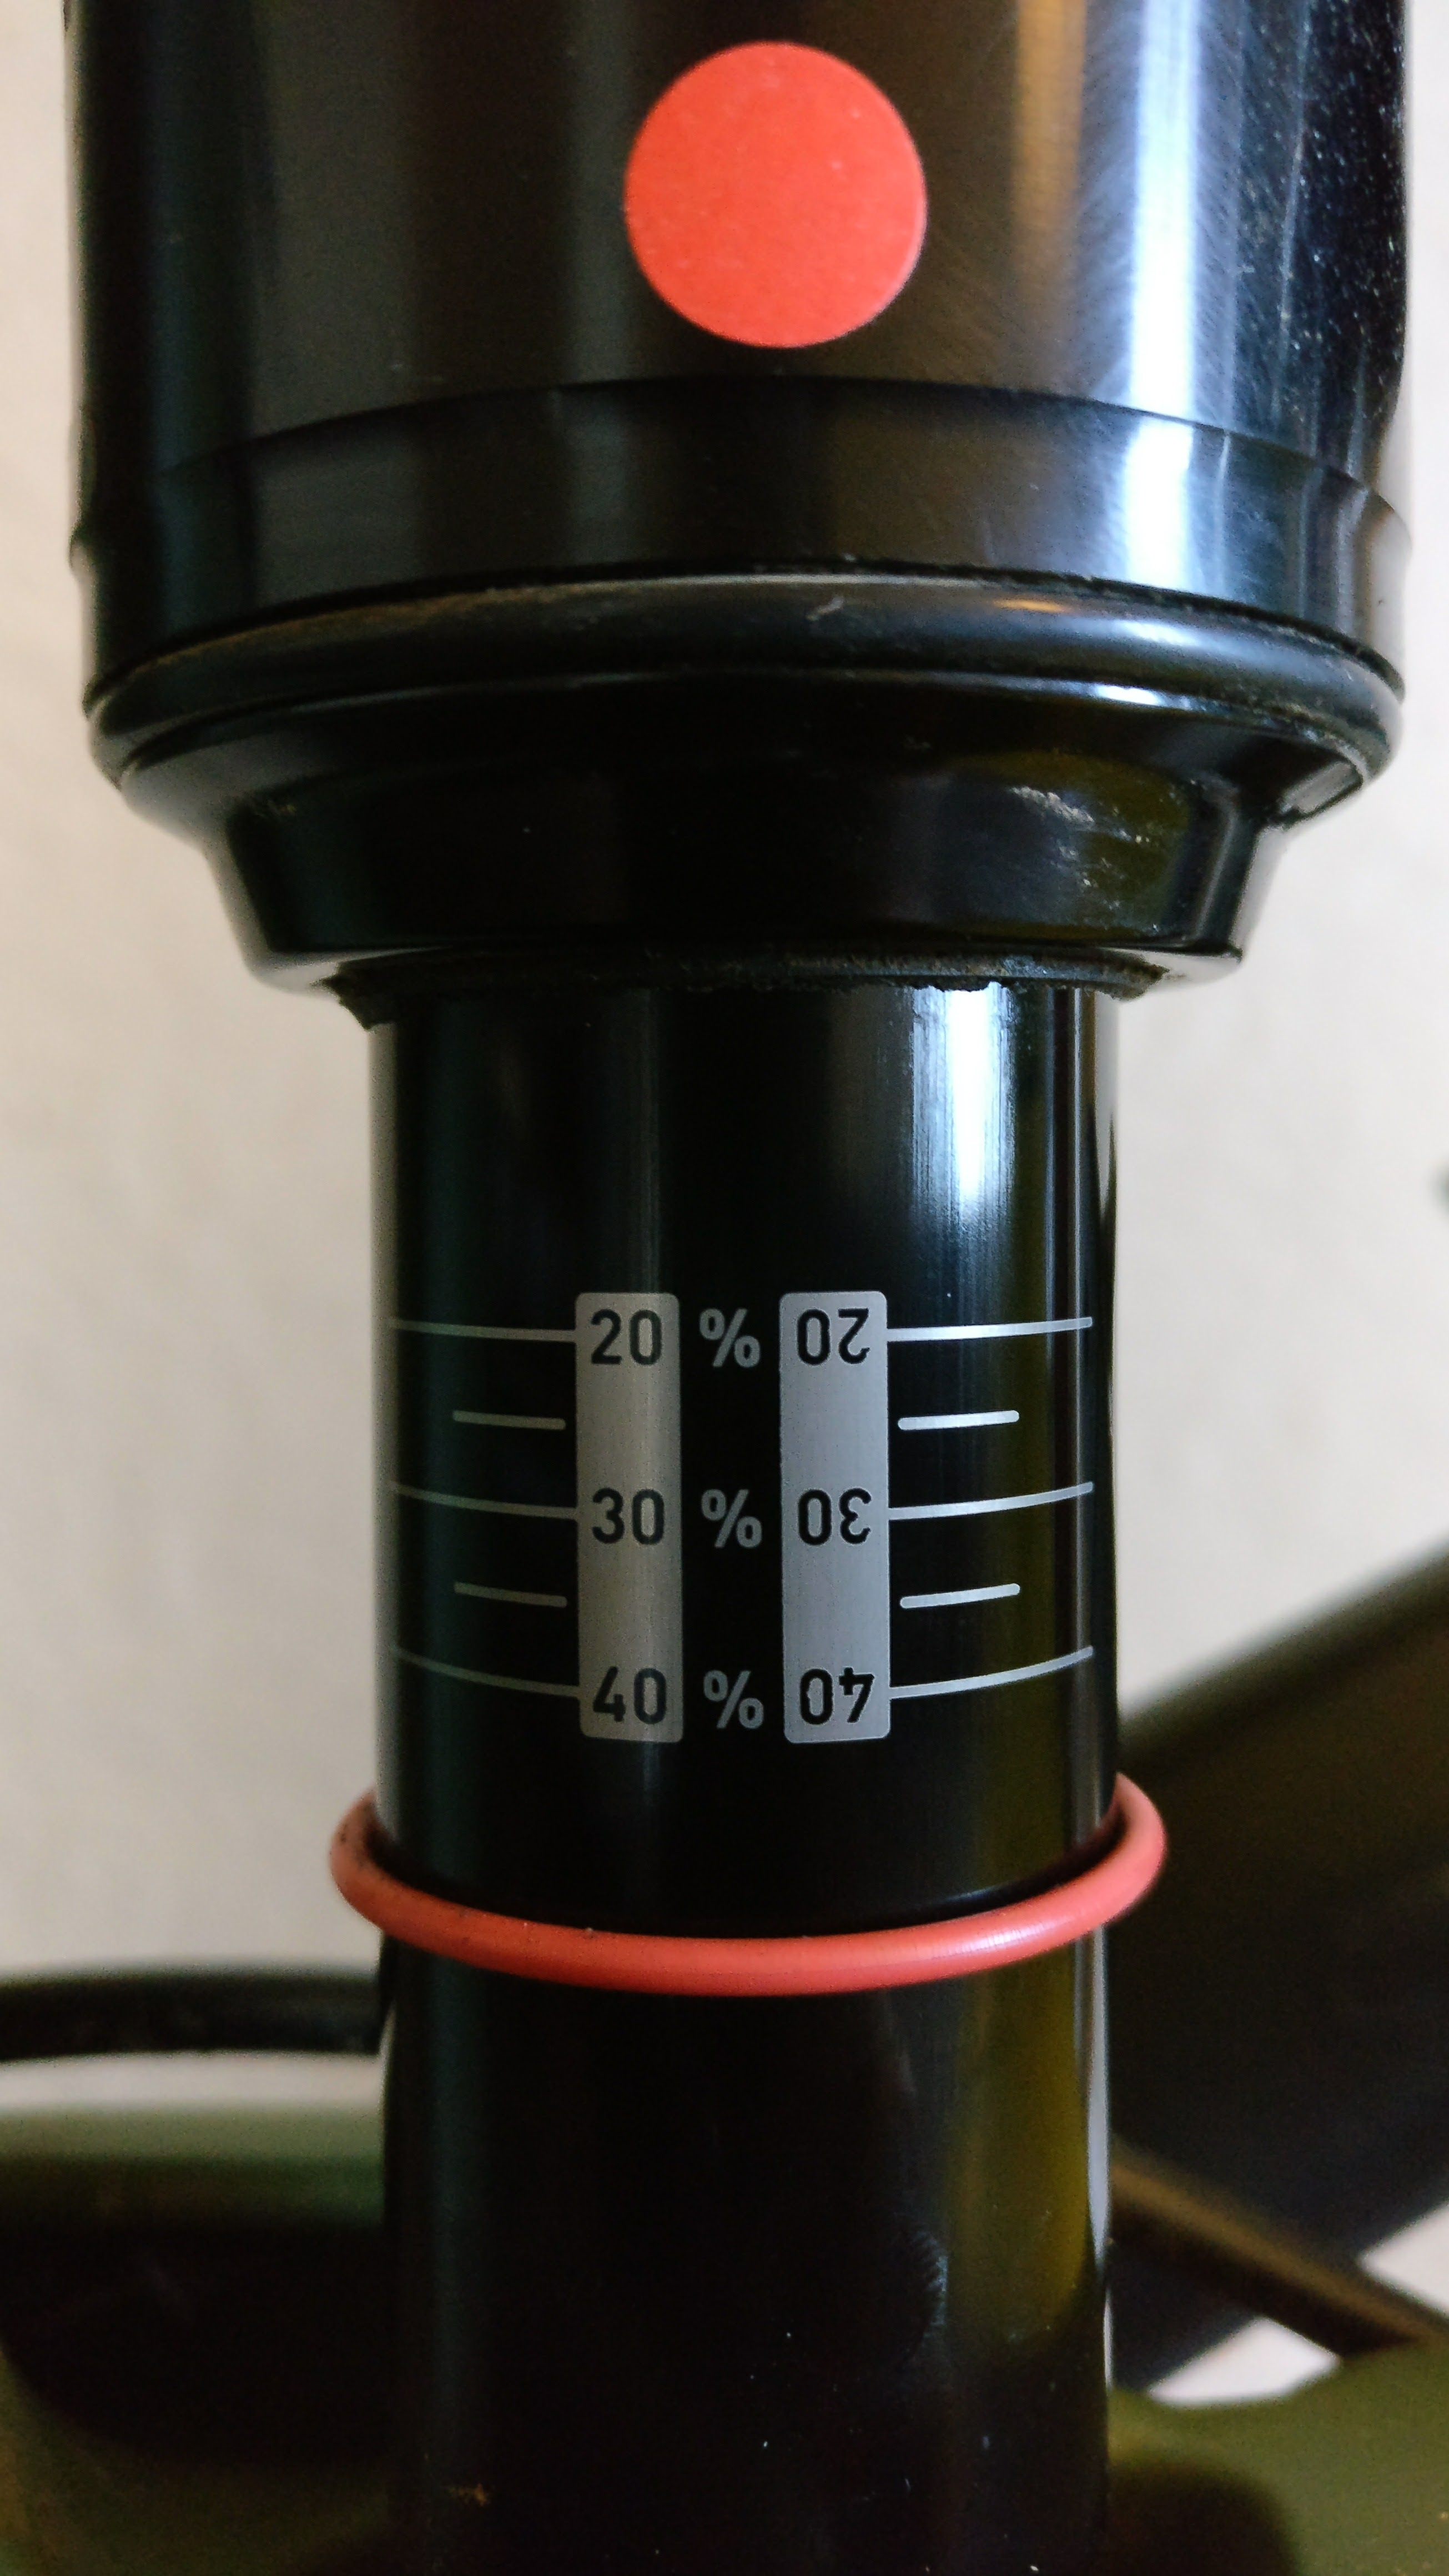
\includegraphics[scale=0.1,trim={0 140cm 0 0}, clip]{../images/results/100_rs.jpg}
			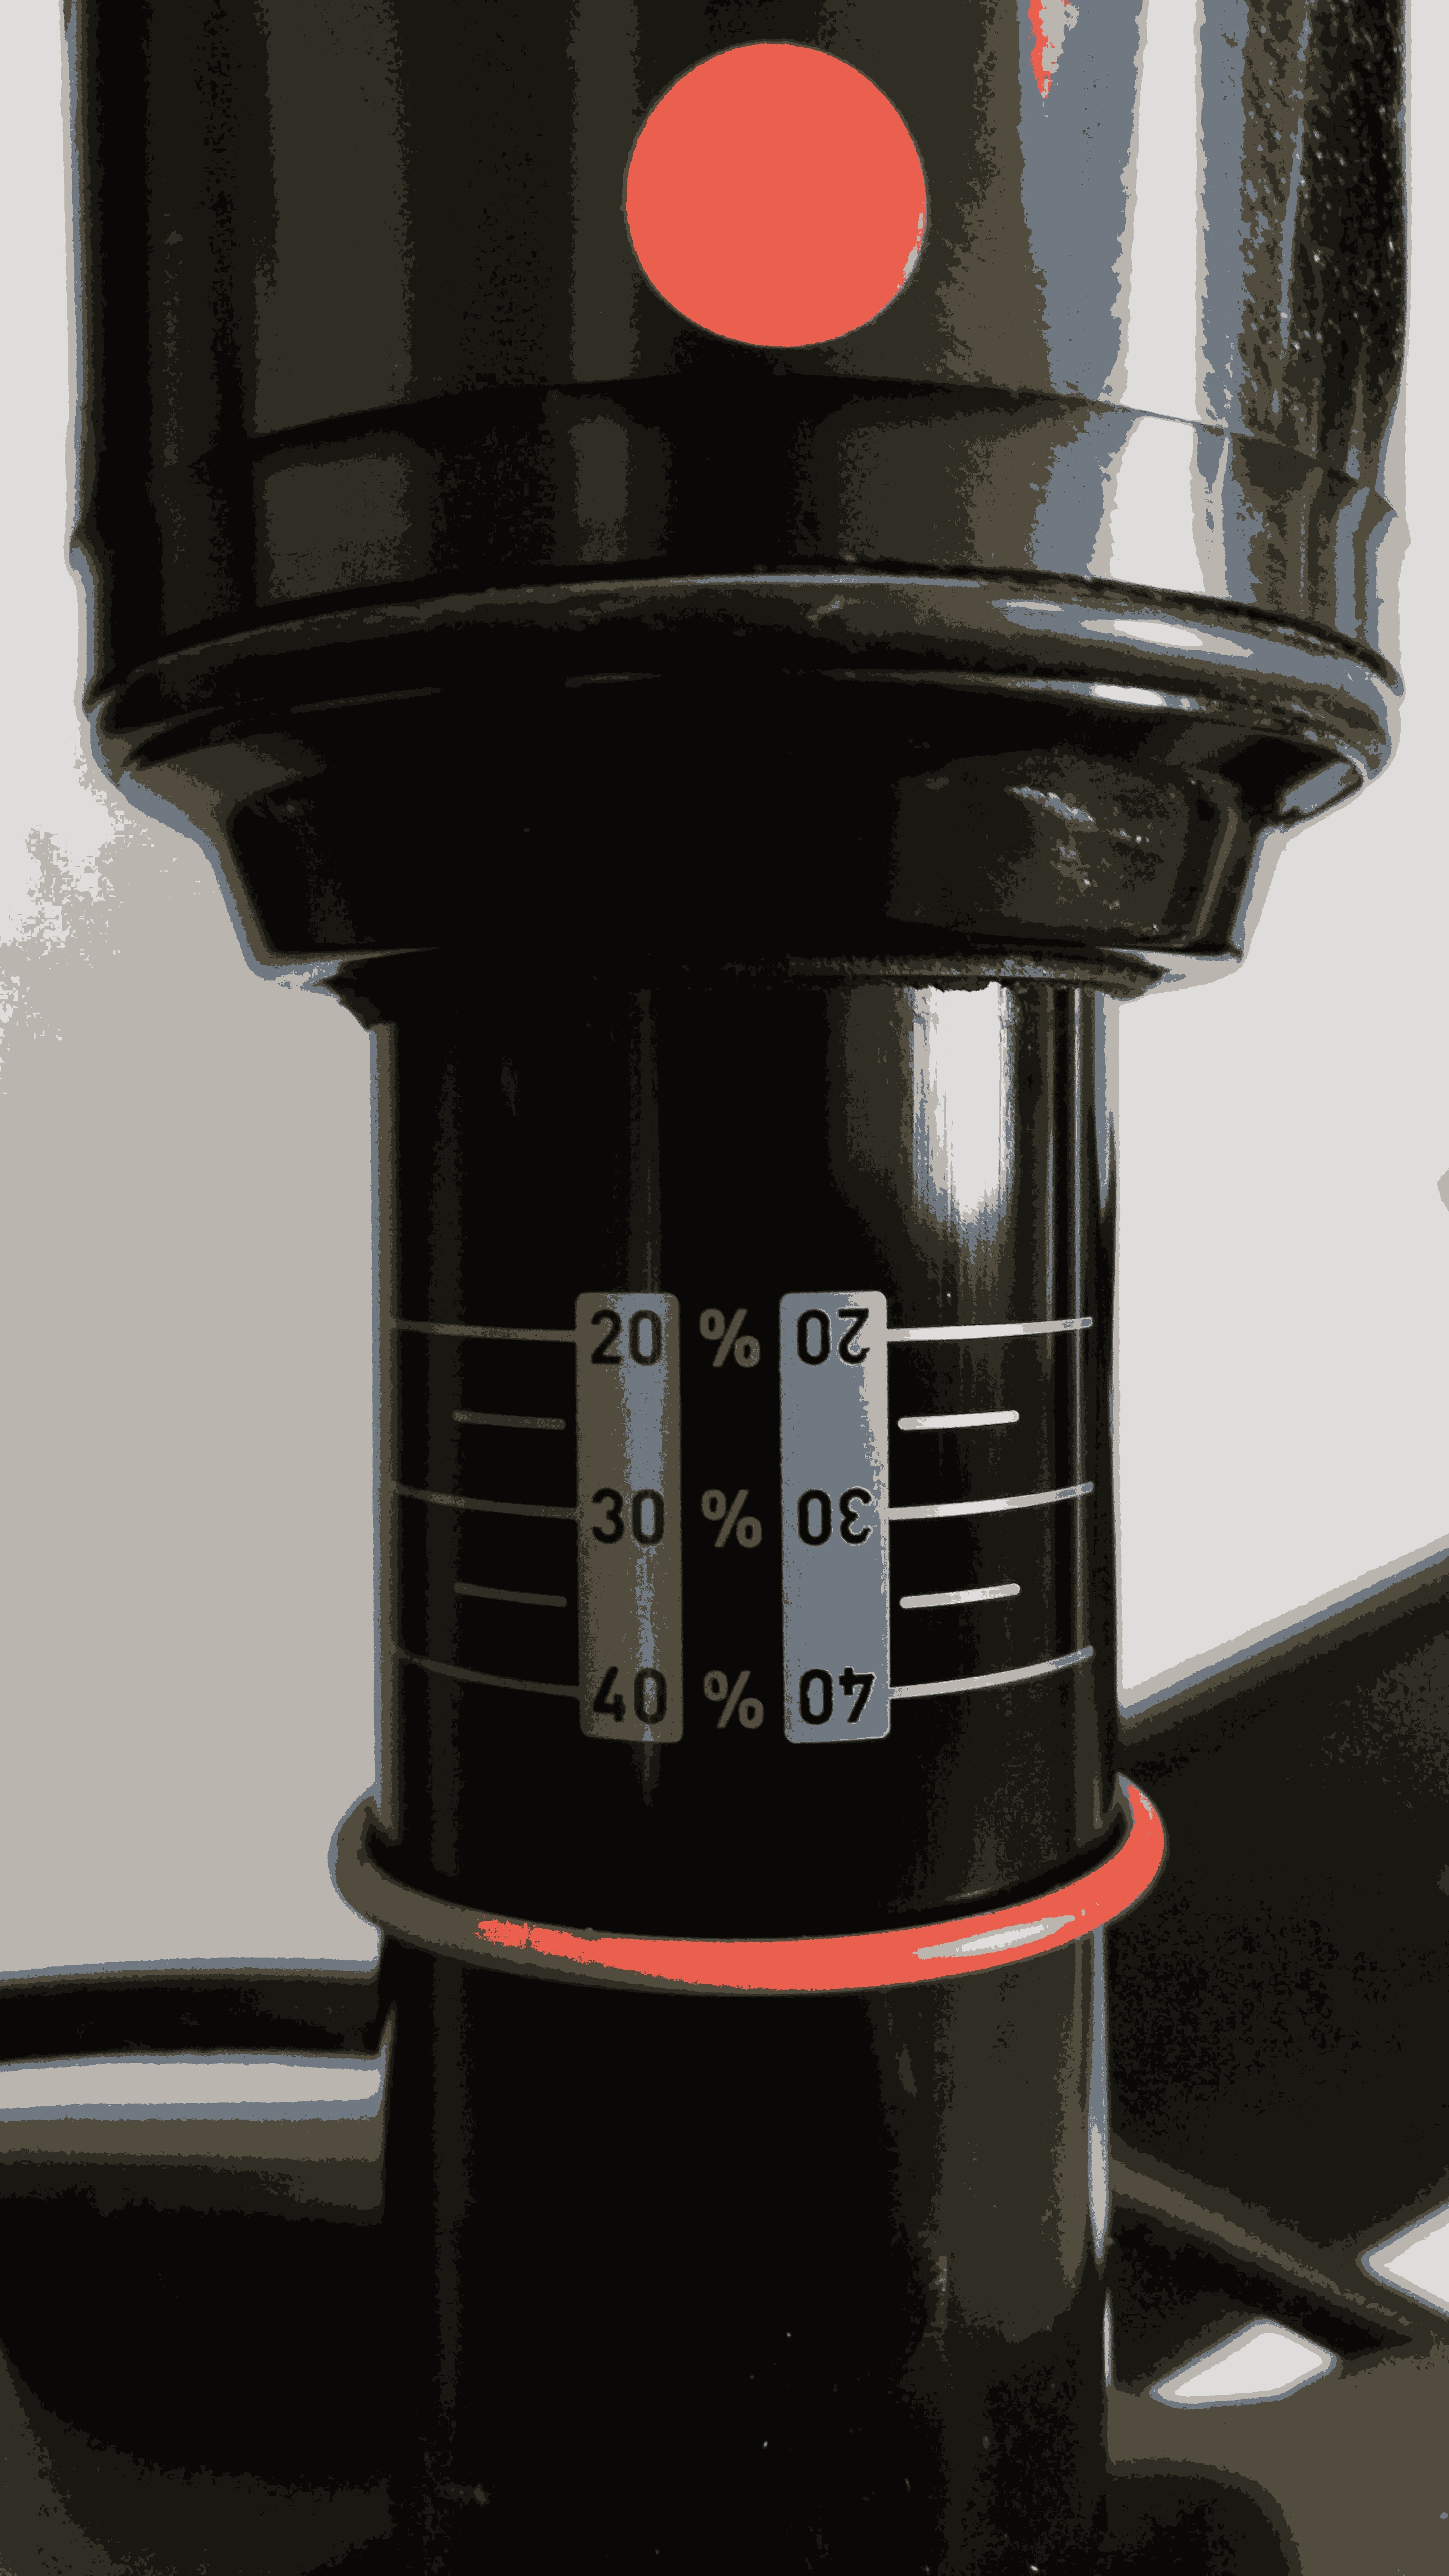
\includegraphics[scale=0.1,trim={0 140cm 0 0},clip]{../images/results/quant.jpg}
			\caption{Normal image (top) versus quantified colours (bottom)}
			\label{fig:quantified_colours}
		\end{figure}
	\subsubsection{Dynamic Measurement Limits}
		It was decided that the application should utilise the distance between the shock wiper seal and the marker o-ring for providing the measurement. This was deemed suitable as the manual process to calculate sag also uses the o-ring and it should be present on most shocks; the only reasons an o-ring would not be present is if it has been removed by the owner. Initial versions of the application assumed the o-ring was positioned around 2/3 of the image height though once multiple images were used from two different shocks this assumption was no longer correct.
		\\\\
		So the application is able to analyse different images, a dynamic method to find this o-ring was implemented. Much like finding the reference point an o-ring of specific colour is found, if present, using OpenCV's {\ttfamily findContours}. When located, a bounding box is drawn round the contour from which the y coordinate and height are used to set the limit of measurement. This can be seen in figure \ref{fig:find_oring}.
		\begin{figure}[h!]
			\centering
			\begin{minipage}{0.4\textwidth}
				\centering
				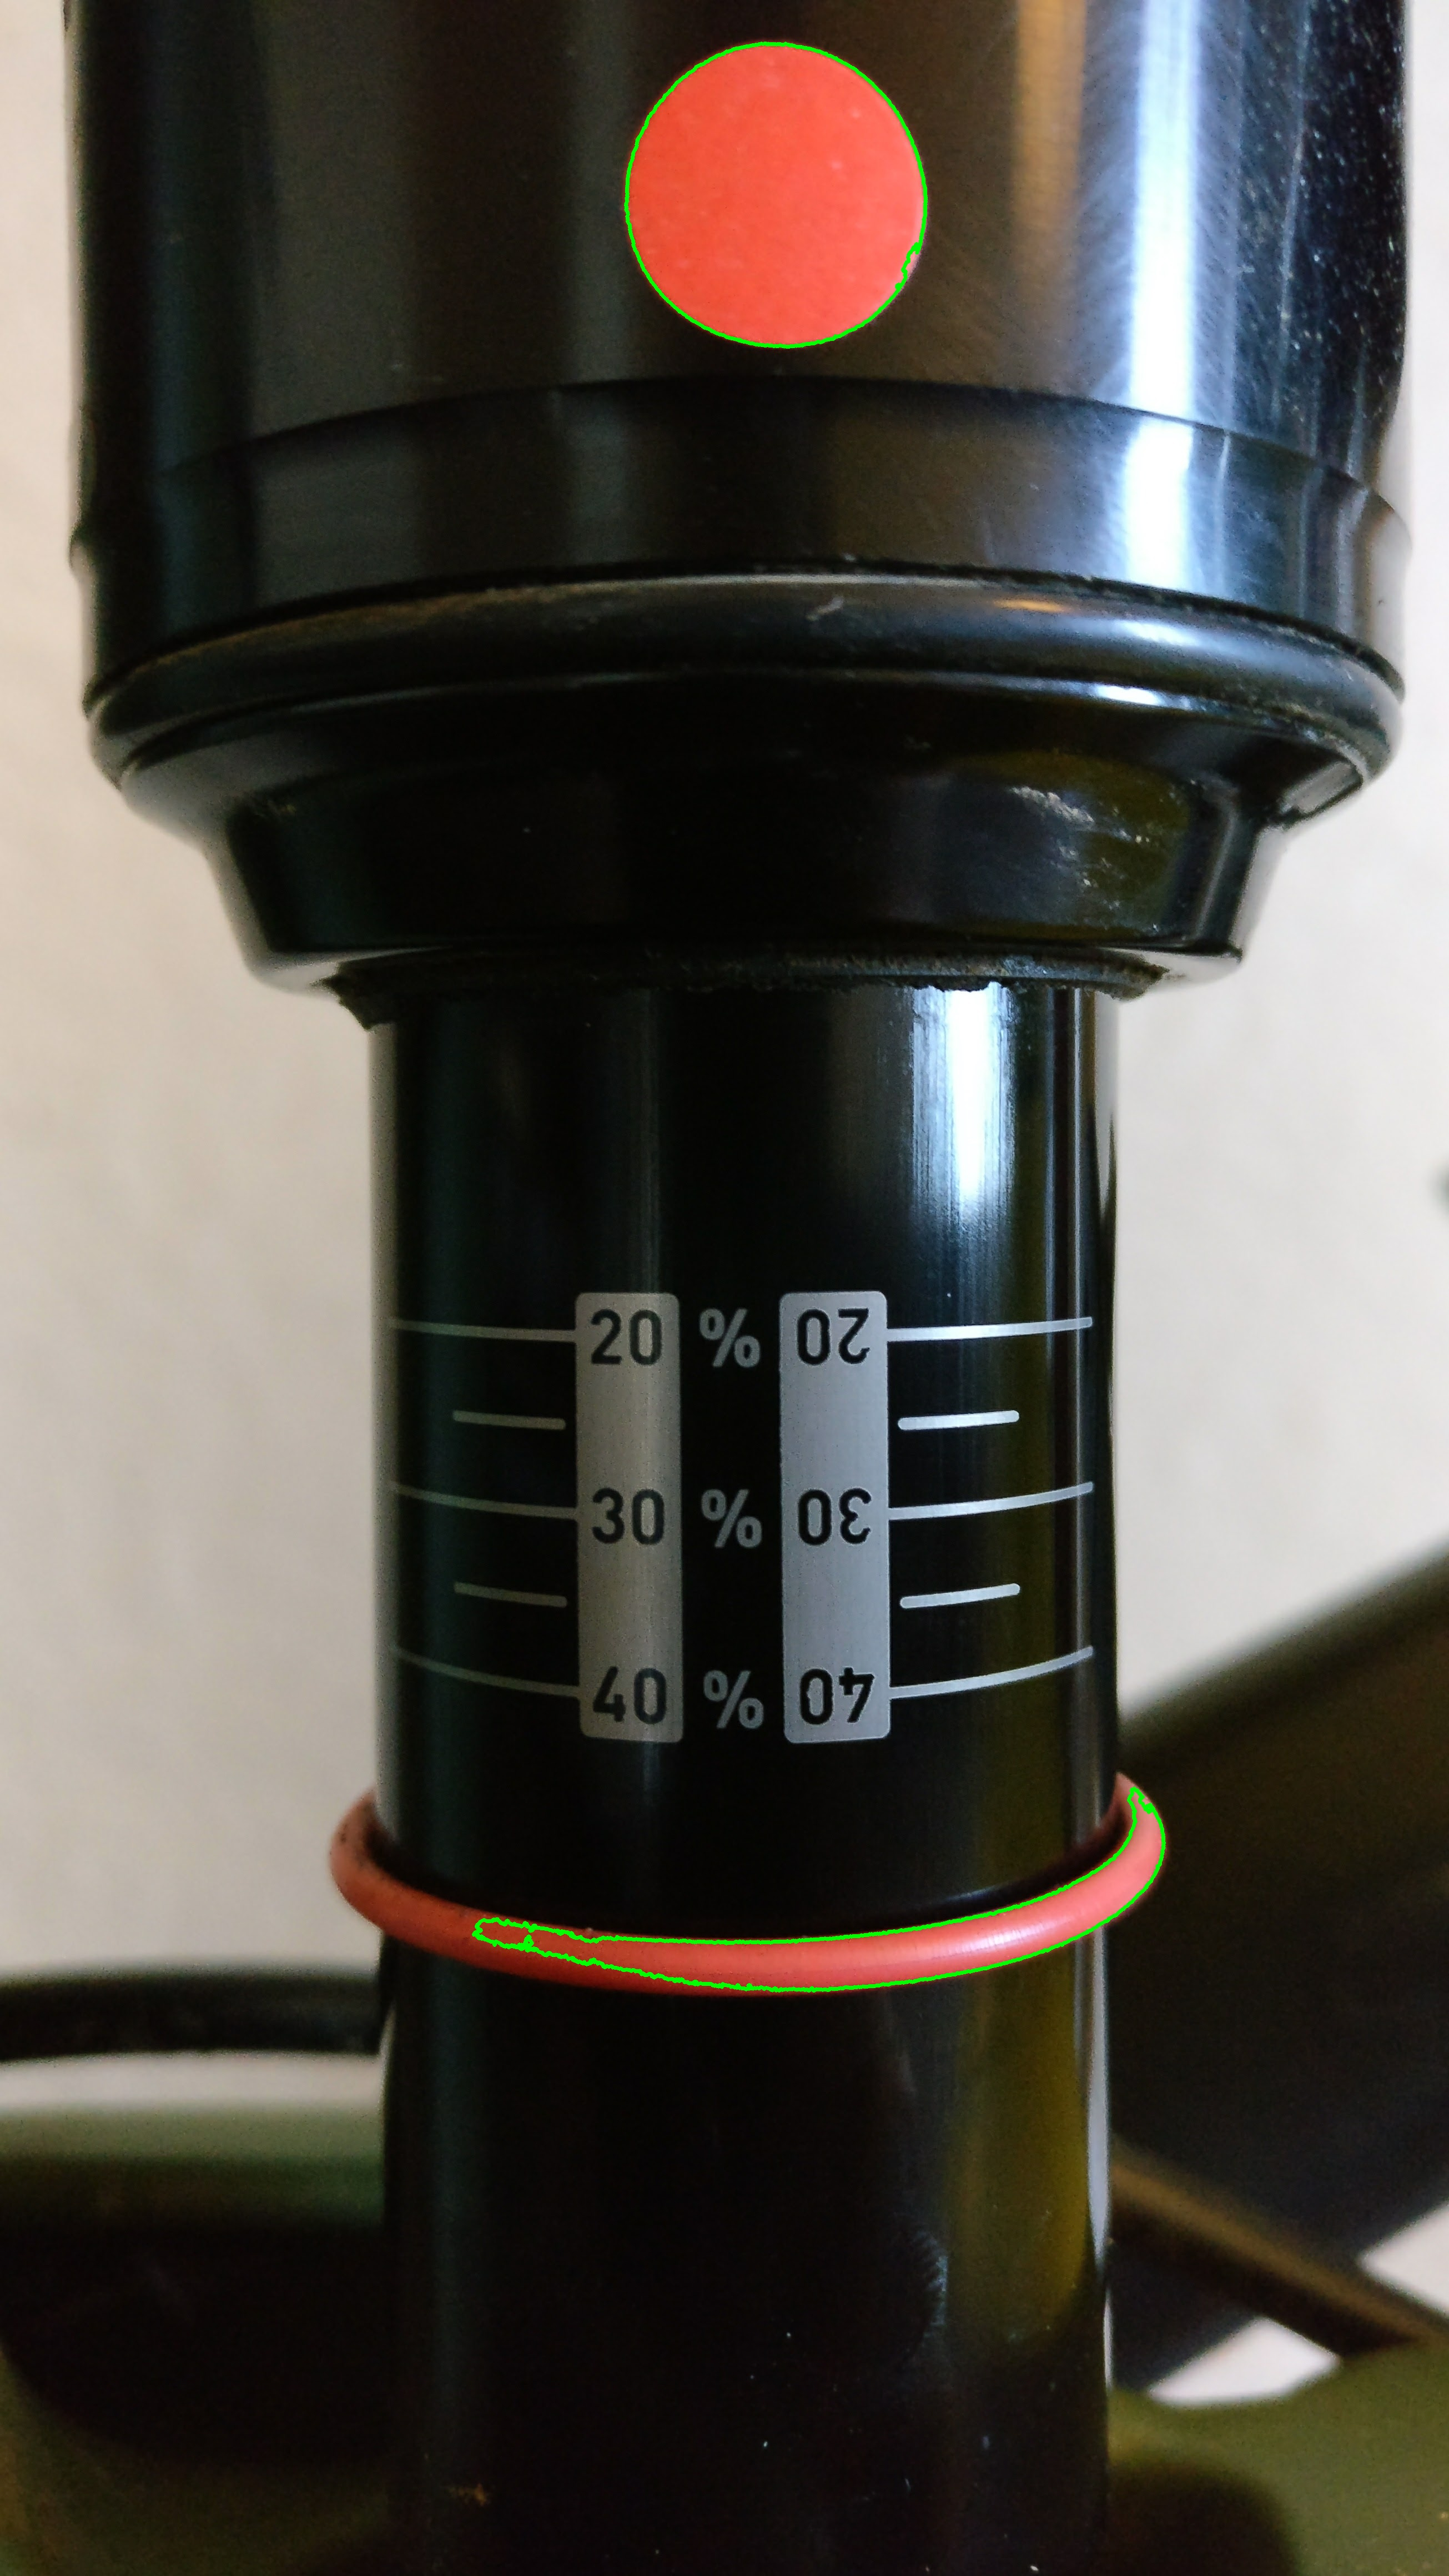
\includegraphics[scale=0.1,
					trim={20cm 30cm 15cm 110cm},
					clip]{../images/results/contours.jpg}				
			\end{minipage}
			\begin{minipage}{0.4\textwidth}
				\centering
				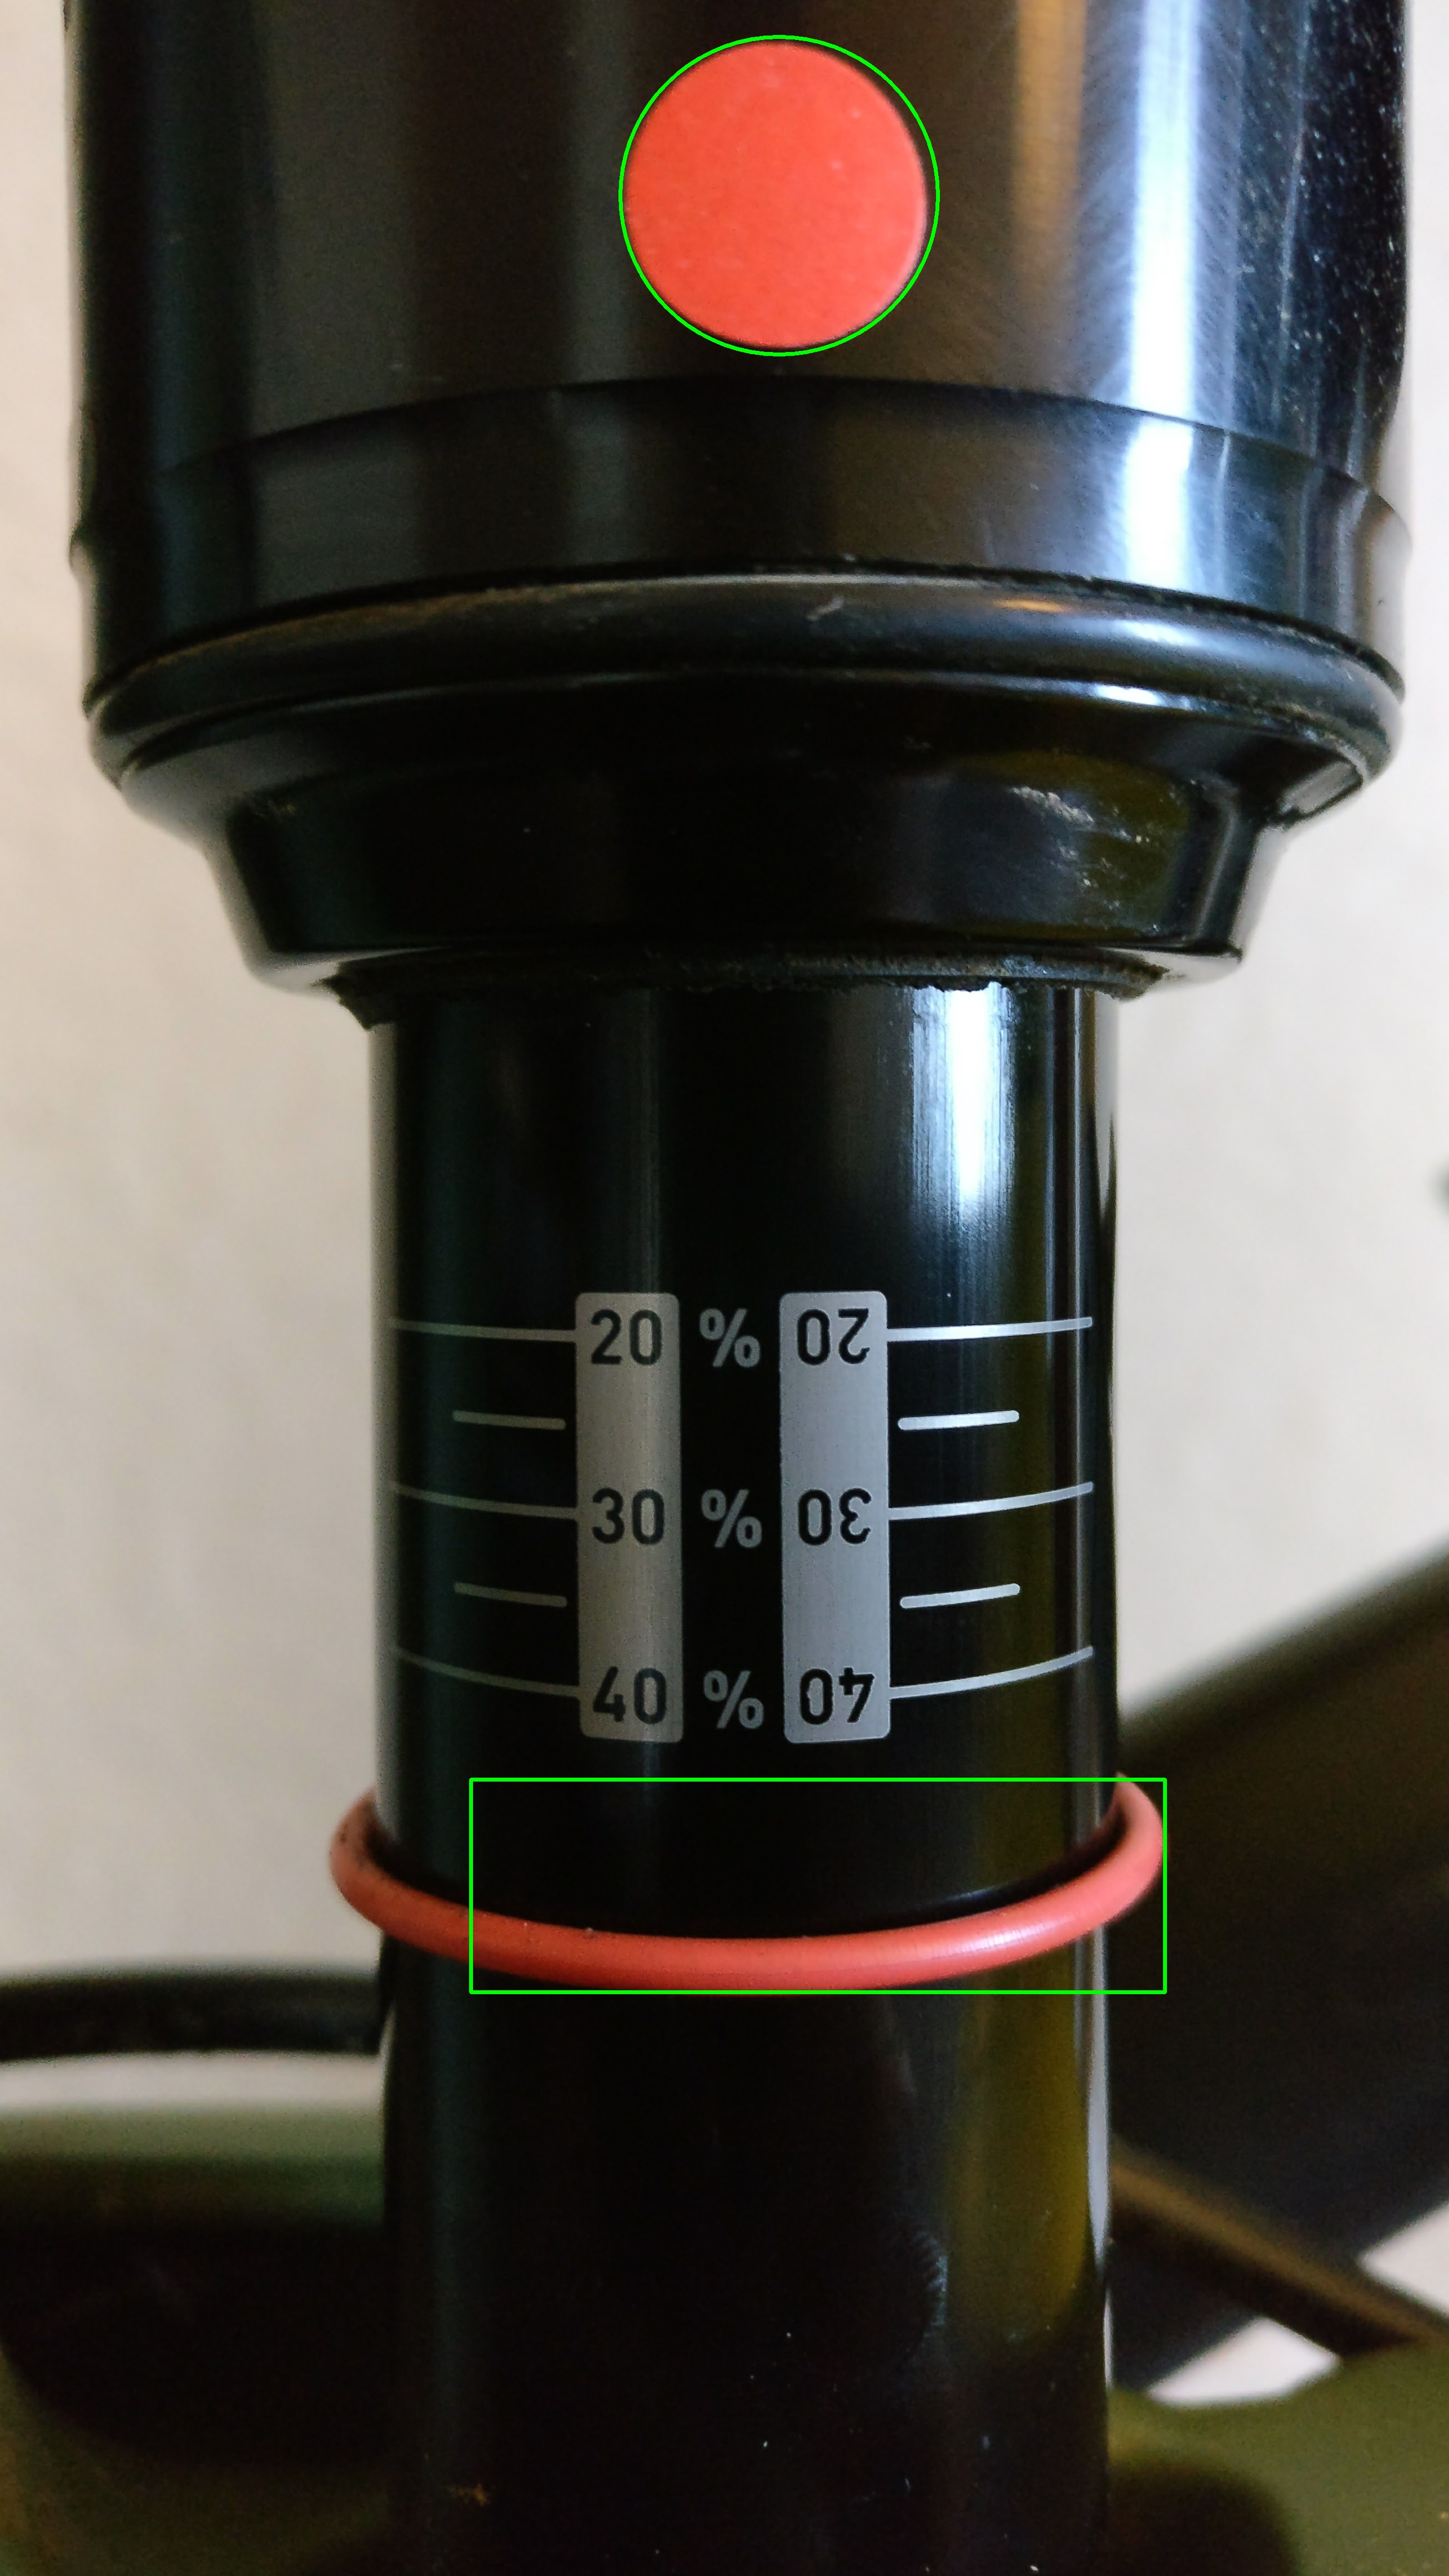
\includegraphics[scale=0.1,
					trim={20cm 30cm 15cm 110cm},
					clip]{../images/results/raw_refs.jpg}				
			\end{minipage}\hfill
			\caption{Red O-ring found using {\ttfamily findContours} (left) with {\ttfamily boundingBox} applied (right)}
			\label{fig:find_oring}
		\end{figure}
		\\\\
		As some shocks do not have a coloured o-ring, this process was adapted to locate a black o-ring though it was unsuccessful. In response, an alternative method was applied where thresholding is applied to the image and contours produced by reflection on the shock's shaft are selected. The same bounding box is applied and used as the measurement limit. This process was successful as indicated in figure \ref{fig:black_oring}.
		\begin{figure}[h!]
			\centering
			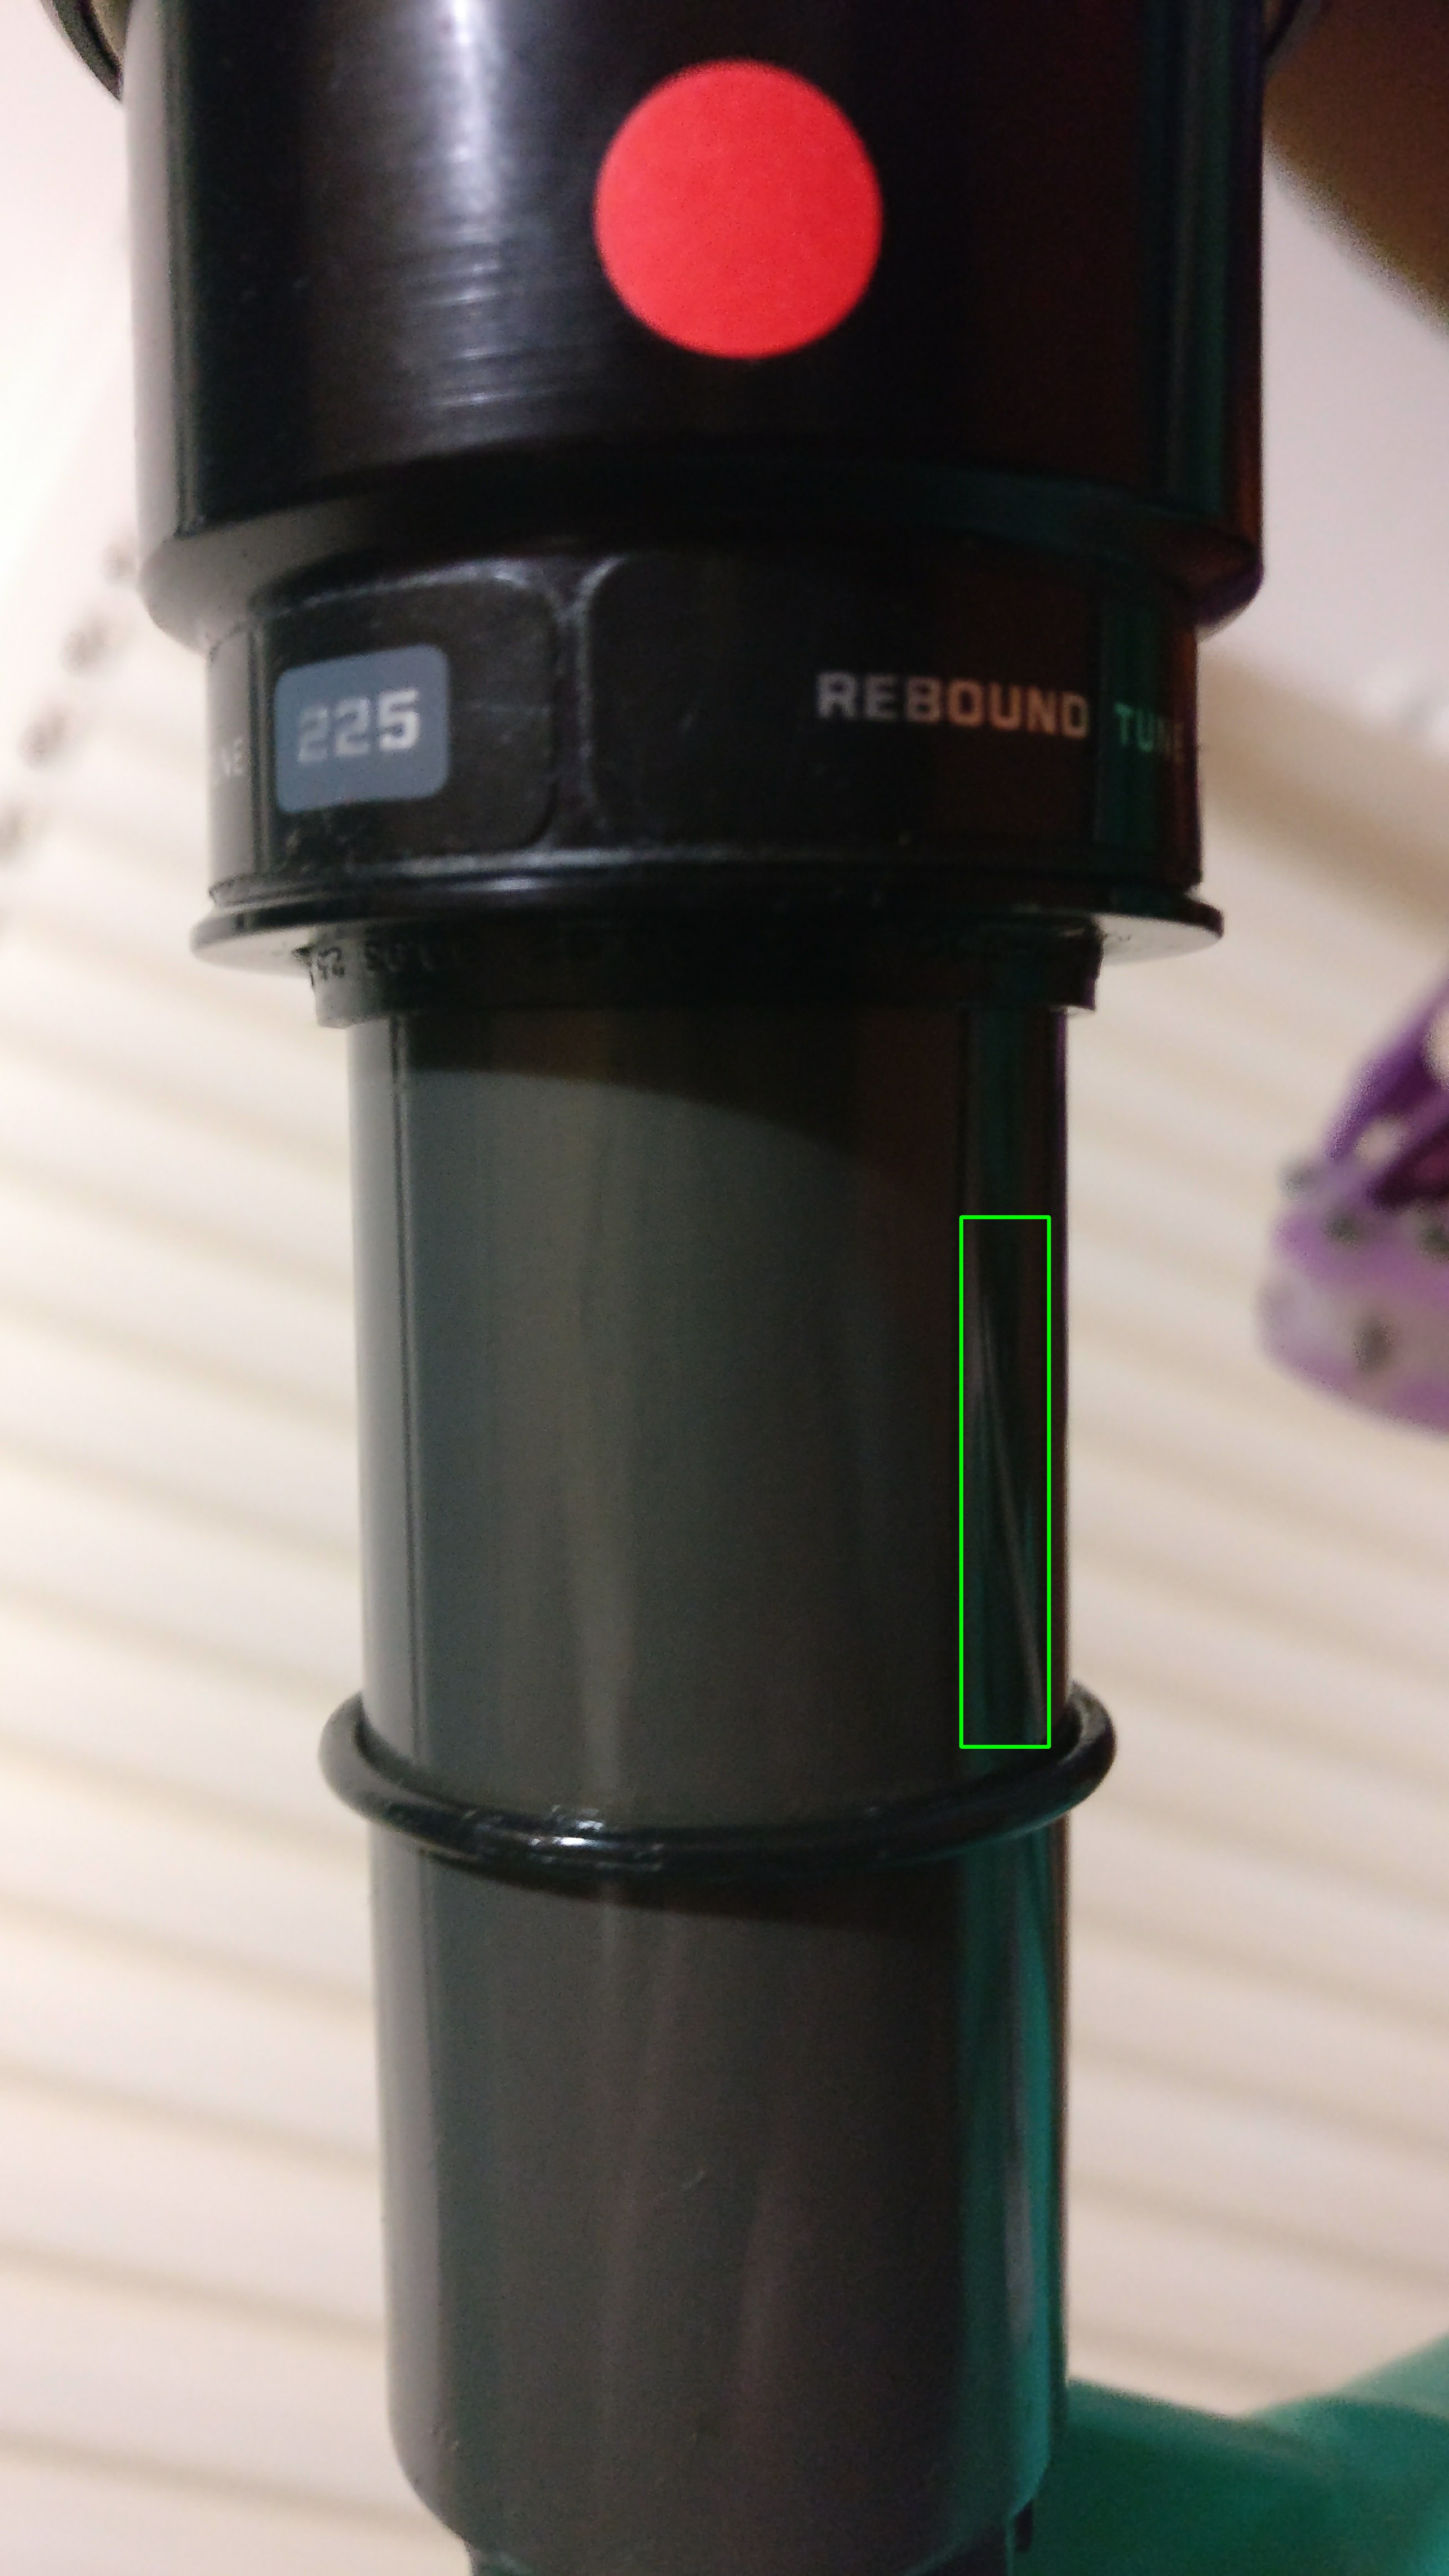
\includegraphics[scale=0.1,trim={20cm 40cm 20cm 70cm},clip]{../images/results/fox_oring.jpg}
			\caption{Black o-ring found}
			\label{fig:black_oring}
		\end{figure}
	\subsubsection{Reference Point Measurement Method}
		To measure the circular reference point, the first process applied was Hough Circle Transform. This method was chosen as it sets out to specifically find circles in an image and is simple to implement. Though this did produce a measurement the numbers were regularly incorrect when compared to manually measuring the image and were unreliable, varying between too small and too big. This can be seen in figure \ref{fig:hough_circle} where it is clear that the identified circle is much smaller than the actual reference point.
		\begin{figure}[h!]
			\centering
			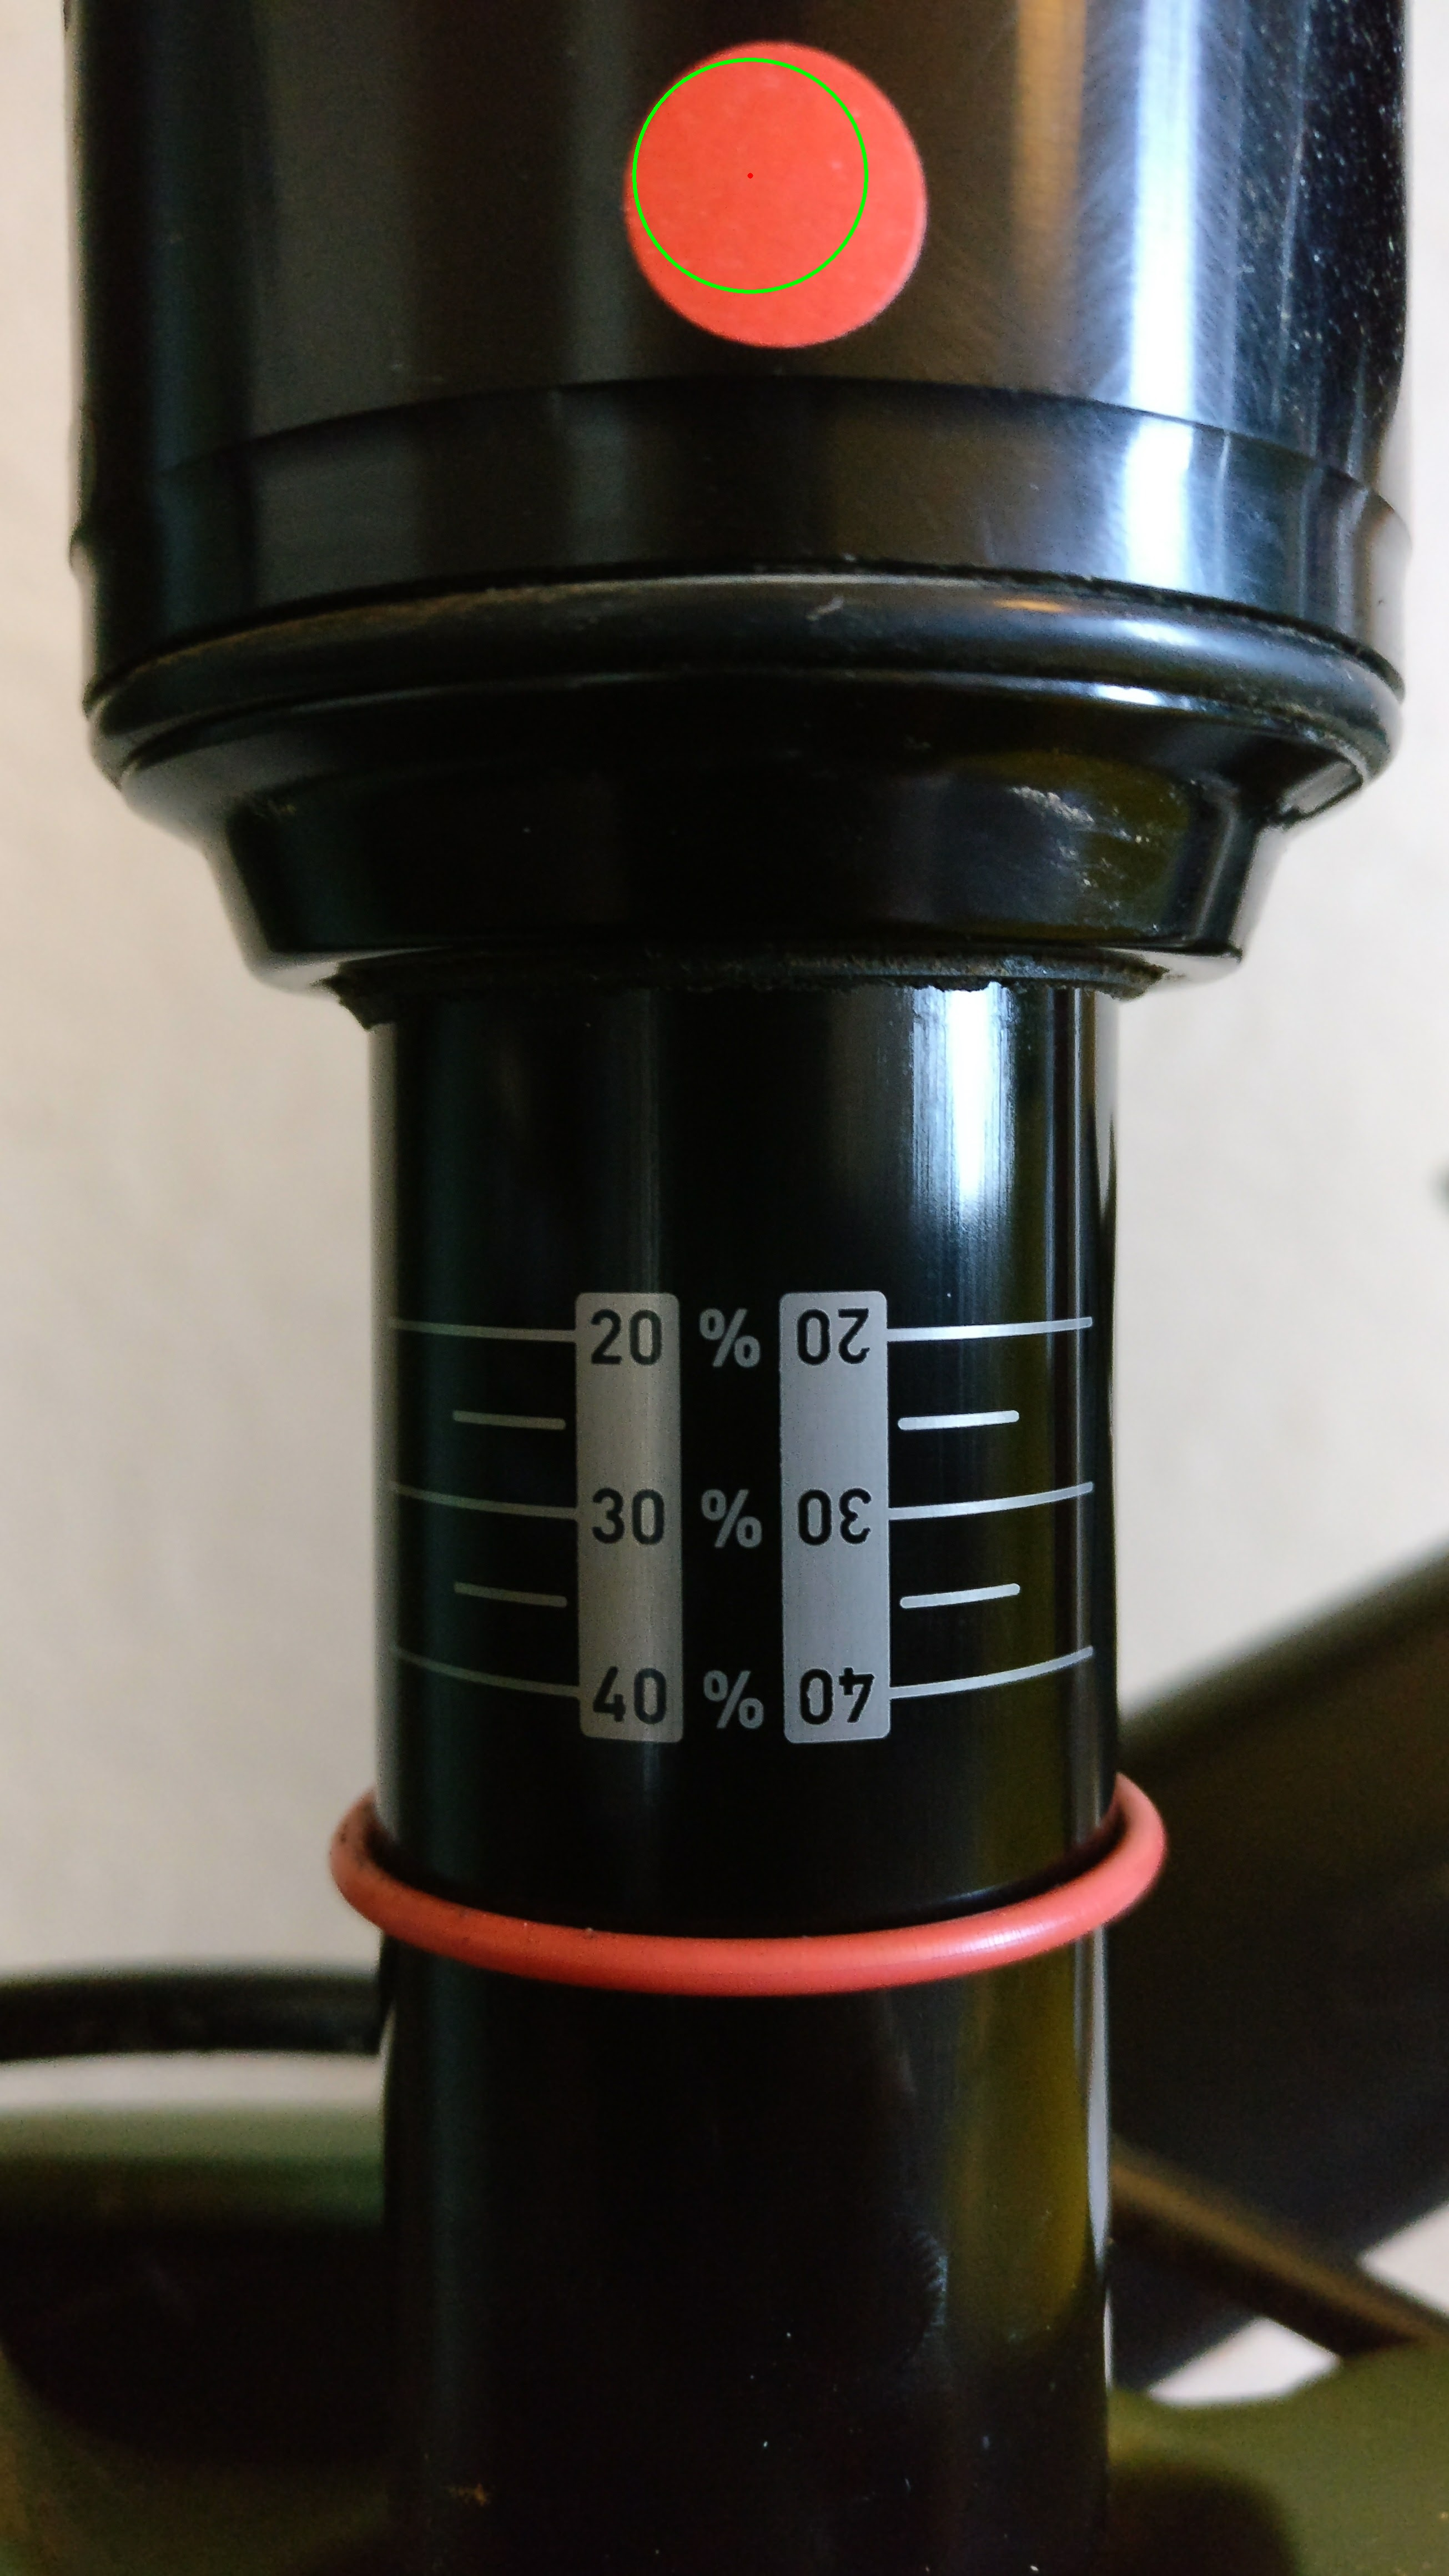
\includegraphics[scale=0.1,
				trim={30cm 140cm 25cm 0},
				clip]{../images/results/HoughCircles.jpg}
			\caption{Reference point found using HoughCircles}
			\label{fig:hough_circle}
		\end{figure}
		\\
		To circumvent this issue the same process for locating the o-ring was used. A contour is found which encompasses the full reference point and a bounding circle is drawn around this contour; this is shown in figure \ref{fig:find_ref}. Though the bounding circle appears larger than the reference point, after experimentation with a variety of images, this method produced measurements which were within tolerances of what is suitable for the pixel per millimetre calculation. 
		\\\\
		This larger appearance is caused by the reference point not being a uniform circle which is also the reason the Hough Circle method was unreliable. Although the threshold of the Hough Circle method can be adjusted, the reference point was still too misshapen to be detected correctly.
		\begin{figure}[h!]
			\centering
			\begin{minipage}{0.4\textwidth}
				\centering
				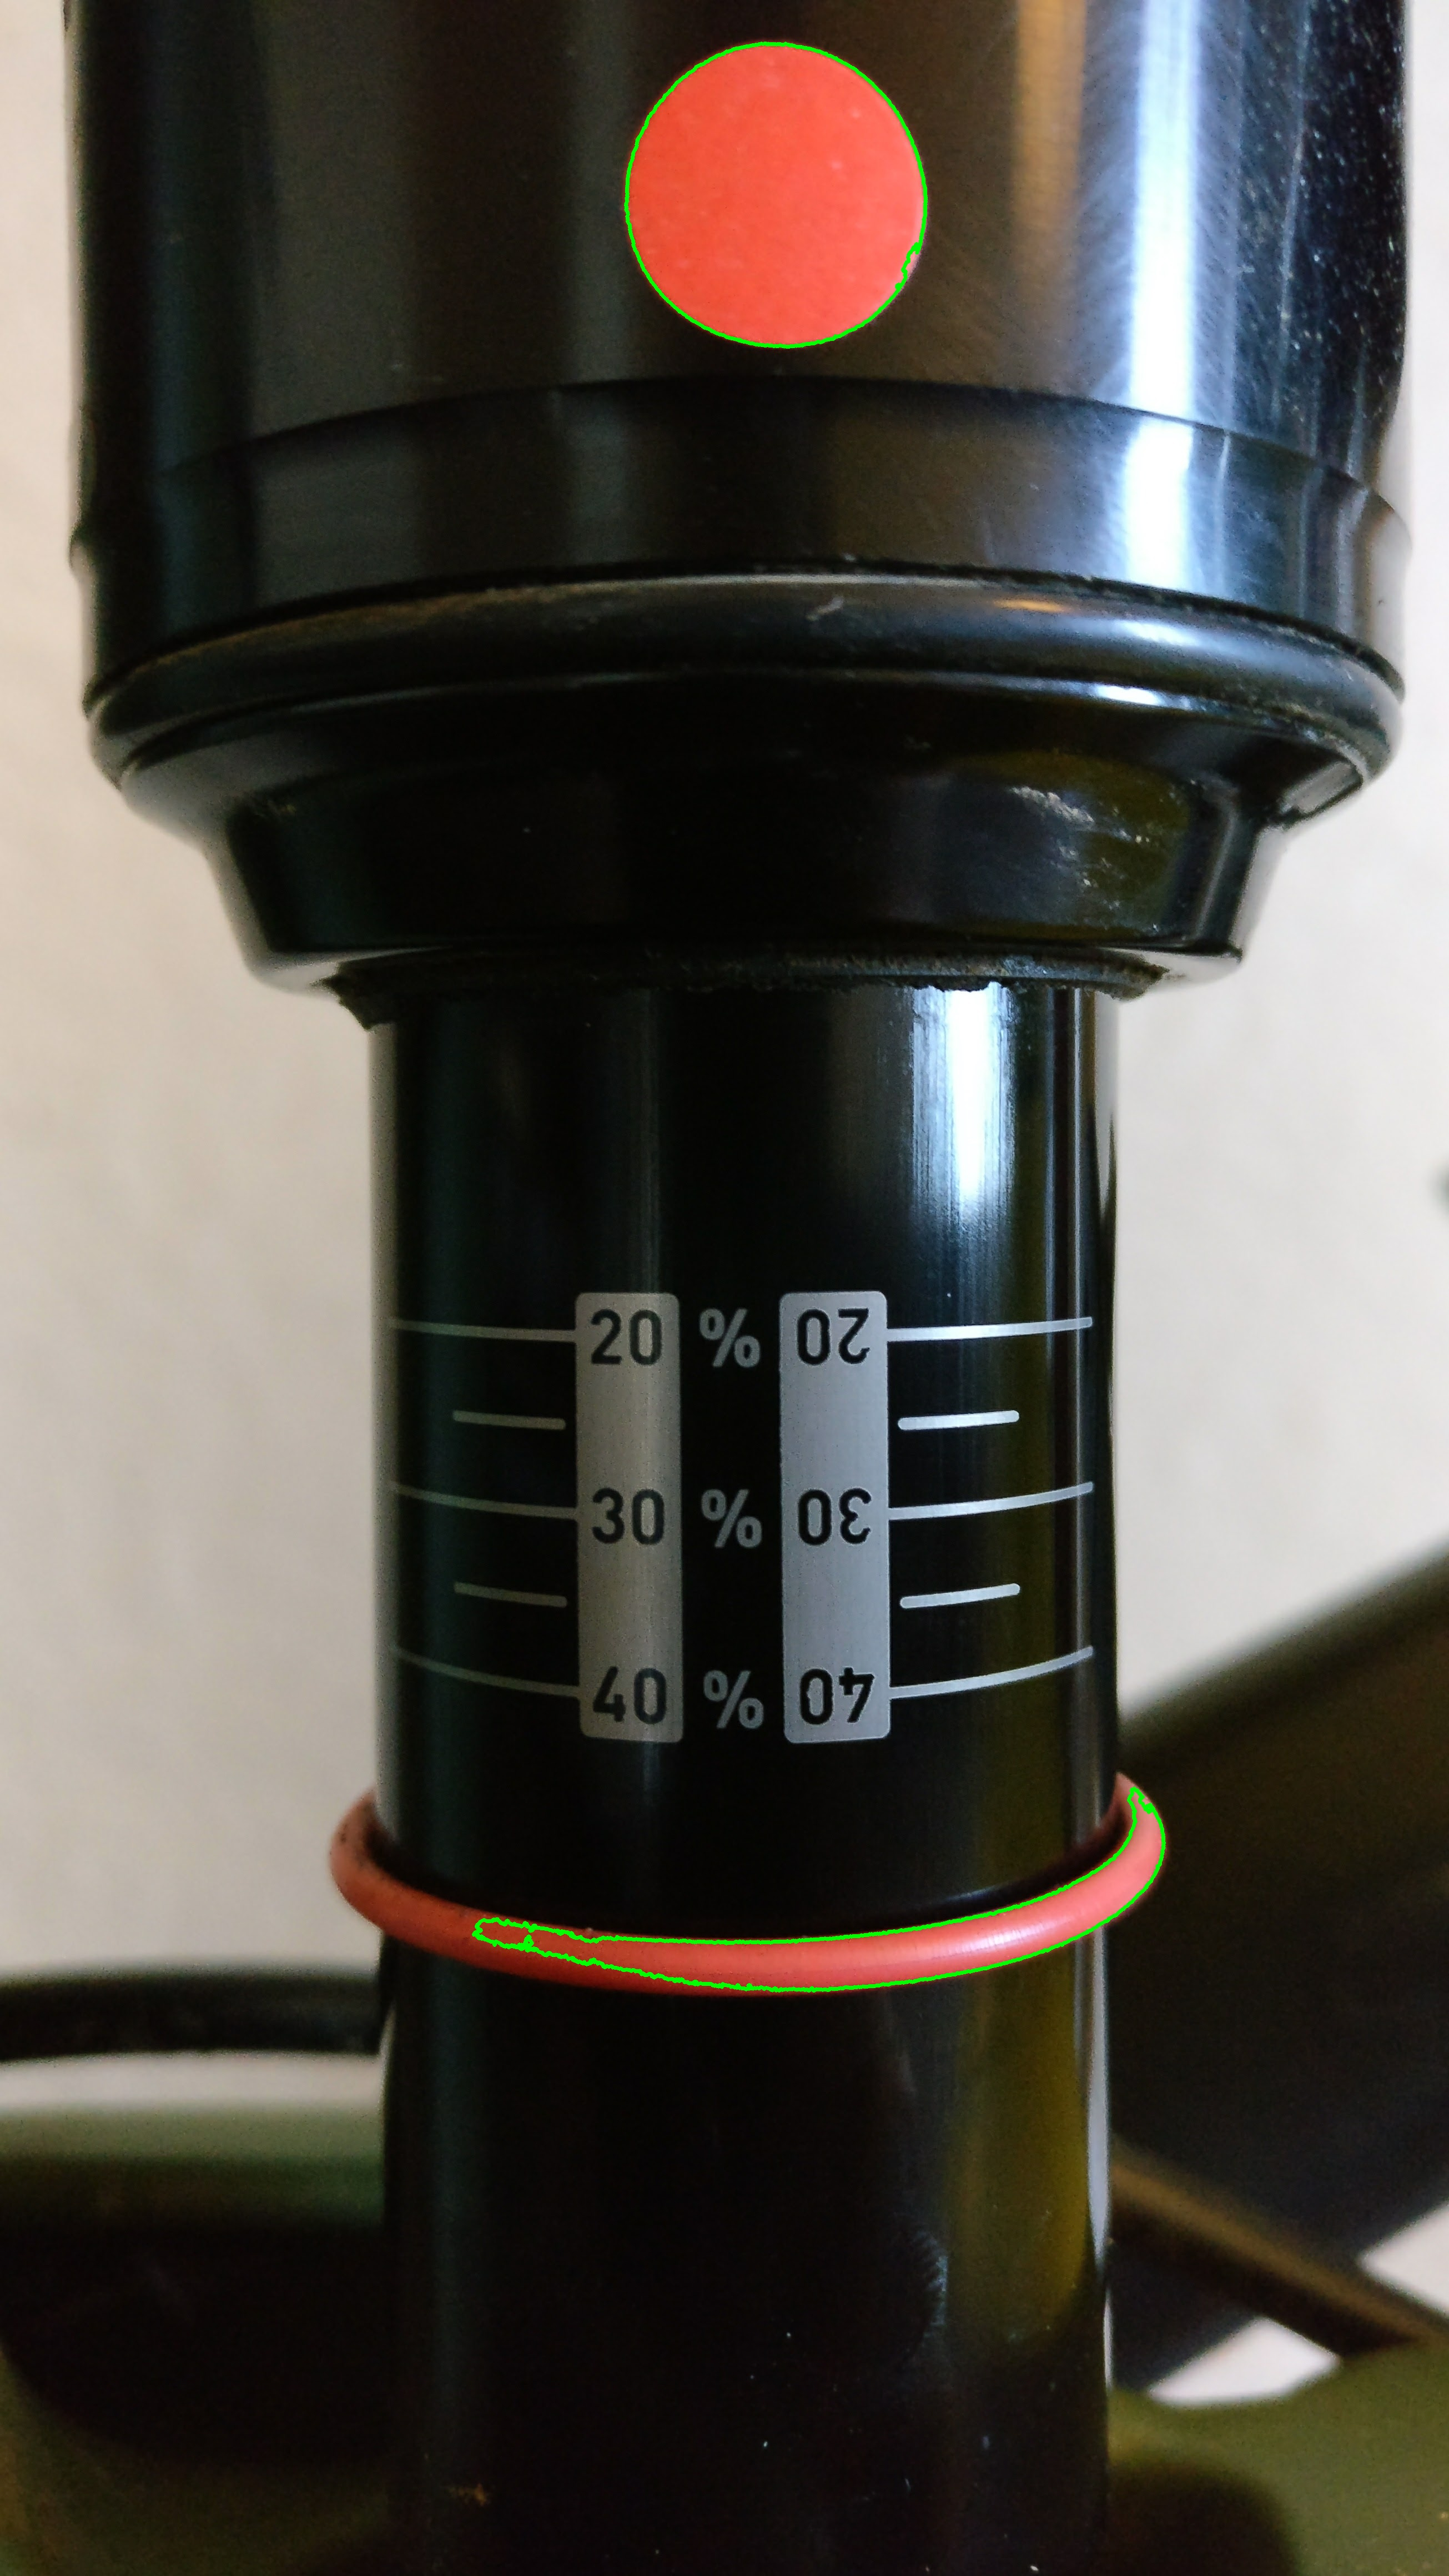
\includegraphics[scale=0.1,
					trim={30cm 140cm 25cm 0},
					clip]{../images/results/contours.jpg}				
			\end{minipage}
			\begin{minipage}{0.4\textwidth}
				\centering
				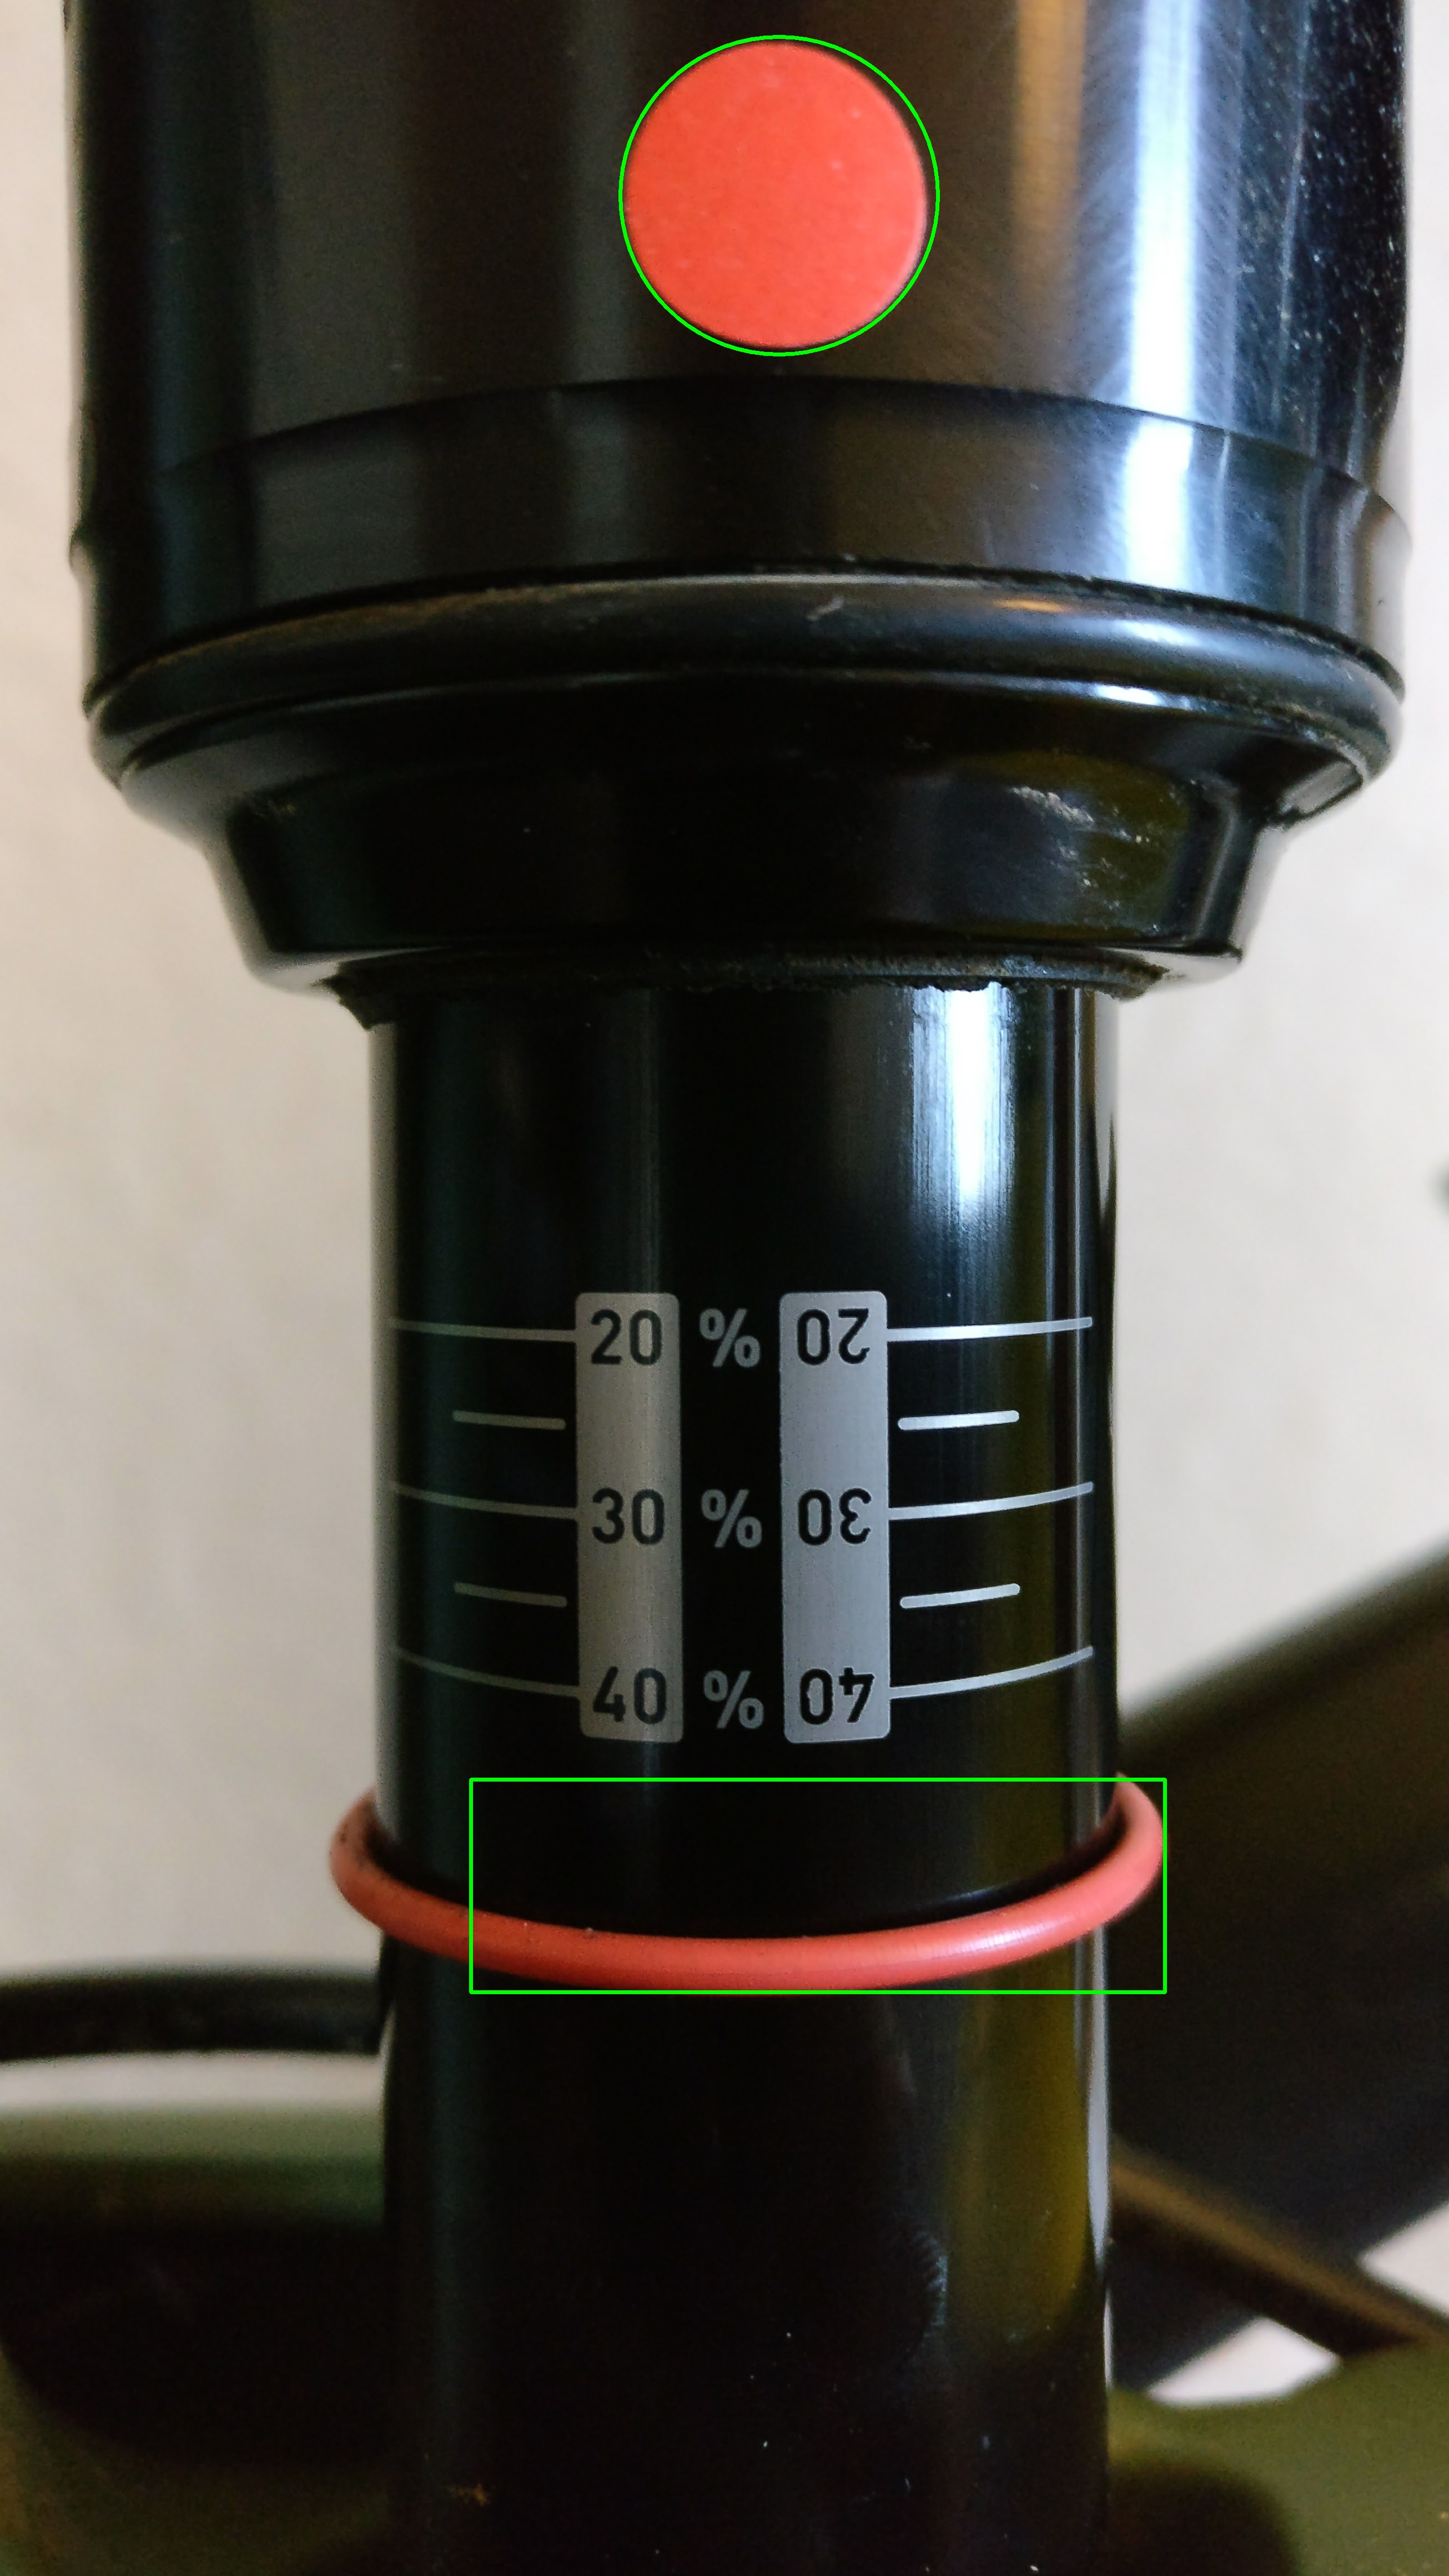
\includegraphics[scale=0.1,
					trim={30cm 140cm 25cm 0},
					clip]{../images/results/raw_refs.jpg}				
			\end{minipage}\hfill
			\caption{Reference point found using findContours (left) with boundingCircle applied (right)}
			\label{fig:find_ref}
		\end{figure}
	\subsubsection{Pressure Calculation}
		The original method for producing a suggested pressure was to calculate a psi per millimetre metric from the measurement of the shock shaft and the current pressure in the shock supplied by the user. The equation for this metric is as follows:
		\begin{equation}
			\label{equ:measureobj}
			P_s = \Bigg(\frac{P_c}{M_c}\Bigg)M_s
		\end{equation}
		\begin{where}
			\item $P_s$ is the pressure to produce the desired sag setting
			\item $P_c$ is the pressure currently in the shock
			\item $M_s$ is the measurement to produce the desired sag setting
			\item $M_c$ is the current measurement of the shock shaft
		\end{where}
		\vspace{5mm}
		Though this hypothesised method had been tested manually on paper with successful results, when implemented within the application it was unable to produce correct settings from any variation of image, reference point, and desired sag even when these values were hard-coded. Through further investigation and discussion it was suggested that the non-linearity of air springs was the cause of the problem.
		\\\\
		When an air spring is compressed the spring rate increases through its travel as the particles become compressed together\todo{cite}; while this allows tuning of the shock characteristics it presents difficulty when attempting to apply a linear equation in a non-linear situation. However as the range of measurement in this project is small compared to the full stroke of an air shock it was considered that the spring rate is linear within this range.
		\\\\
		To investigate this, the sag of a shock was measured at pressures between 100 and 250 psi in increments of 10 psi. This was carried out for two shocks, one with a normal air can and another with a high volume air can then the collected data was then plotted and a linear trend line applied. The results of this can be seen in figure \ref{fig:scatters}.
		\begin{figure}[h!]
			\centering
			\begin{minipage}{0.4\textwidth}
				\centering
				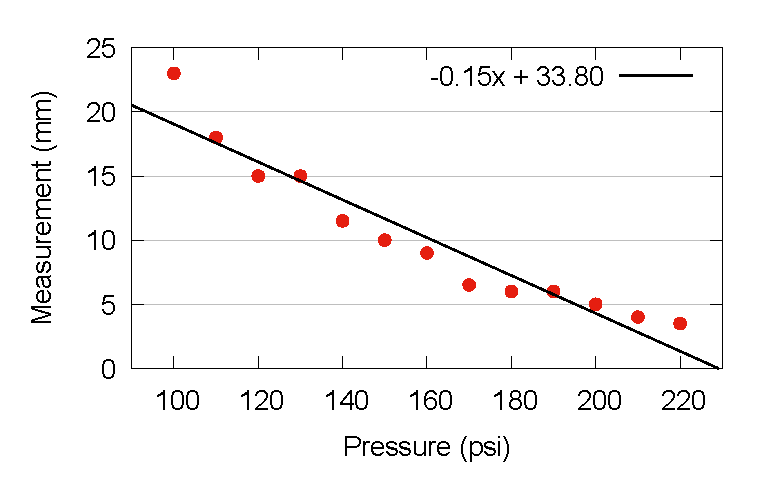
\includegraphics[width=\textwidth]{../images/results/fox_scatter.eps}
			\end{minipage}
			\begin{minipage}{0.4\textwidth}
				\centering
				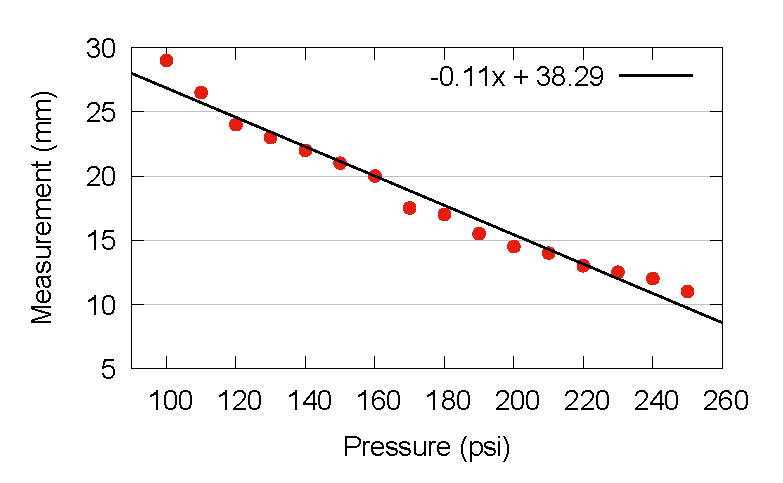
\includegraphics[width=\textwidth]{../images/results/rs_scatter.eps}
			\end{minipage}
			\caption{Sag measurements for standard air shock (left) and high volume air shock (right)}
			\label{fig:scatters}
		\end{figure}\\\\
		From this data it could be concluded that, within the range of measurements, the compression of the air spring is linear. The data-points in figure \ref{fig:scatters} occasionally vary though this is due to a non sterile test. Both shocks were well used potentially containing age related defects and loading the bike was carried out using body weight.
		\\\\
		The plan with this knowledge was to implement an ideal gas equation but through investigation into producing charts using python, a method of calculating a linear equation computationally was discovered. This led to the application's process being rearranged so that it takes in two images, one of the shock loaded at 100psi and another at 150psi. From this data it can produce a virtual plot and linear equation with which the suggested setting can be calculated.
\subsection{Application}
	\subsubsection{Arguments}
		The application operates from a command line interface allowing the user to pass in data through arguments; these are described in Table \ref{tab:arguments}. This system uses Python's Argparse package and a full command to run the application would be as follows:
		{\centering \ttfamily program -i user/images/100.jpg user/images/150.jpg -s 30 -t 57 -c red}
		\begin{table}[h!]
			\centering
			\caption{Table of application arguments}
			\label{tab:arguments}
			\begin{tabular}{|l|p{0.35\columnwidth}|p{0.25\columnwidth}|}
			\hline
			\bfseries Argument&\bfseries Description&\bfseries Usage\\
			\hline
			{\ttfamily [-i,--image]<path1 path2>}&The paths to the two images to be used for analysis&{\ttfamily -i path/to/img/1 path/to/img/2}\\
			{\ttfamily [-s,--sag]<percentage>}&The desired sag percentage&{\ttfamily -s 30}\\
			{\ttfamily -t,--stroke}&The stroke length of the shock being analysed&{\ttfamily -t 57}\\
			{\ttfamily -c,--colour}&The colour of the marker o-ring&{\ttfamily -c red}\\
			{\ttfamily -d,--debug}&This produces outputs from each stage to the terminal for debugging purposes&\\
			\hline
			\end{tabular}
		\end{table}
	\subsubsection{Process}
		\paragraph{Reference Point}
			The first process which the application must complete is to find the reference point for measurement. This is done by first colour quantifying the image to 8 bit colour so that the reference point becomes uniform in colour. The result of this process is shown in Figure \ref{subfig:quantified}. So the application can find the red colour of the reference point within the entire image, a mask is applied for any colour within a range. The output of this process is shown in Figure \ref{subfig:mask}. If an alternative colour reference point were to be used, this colour range could be easily adapted.
			\\\\
			The contours, or shapes, in this image are then found and sorted by their area in decreasing order. By doing this it can be assumed with a high level of confidence that the largest will be the reference point. The found contour can be seen in Figure \ref{subfig:contours}. A bounding circle is created around the reference point contour, shown in Figure \ref{subfig:boundaries}, from which the diameter can be produced which allows the pixels per millimetre metric.
		\begin{figure}[h!]
			\centering
			\begin{subfigure}[t]{0.2\textwidth}
				\centering
				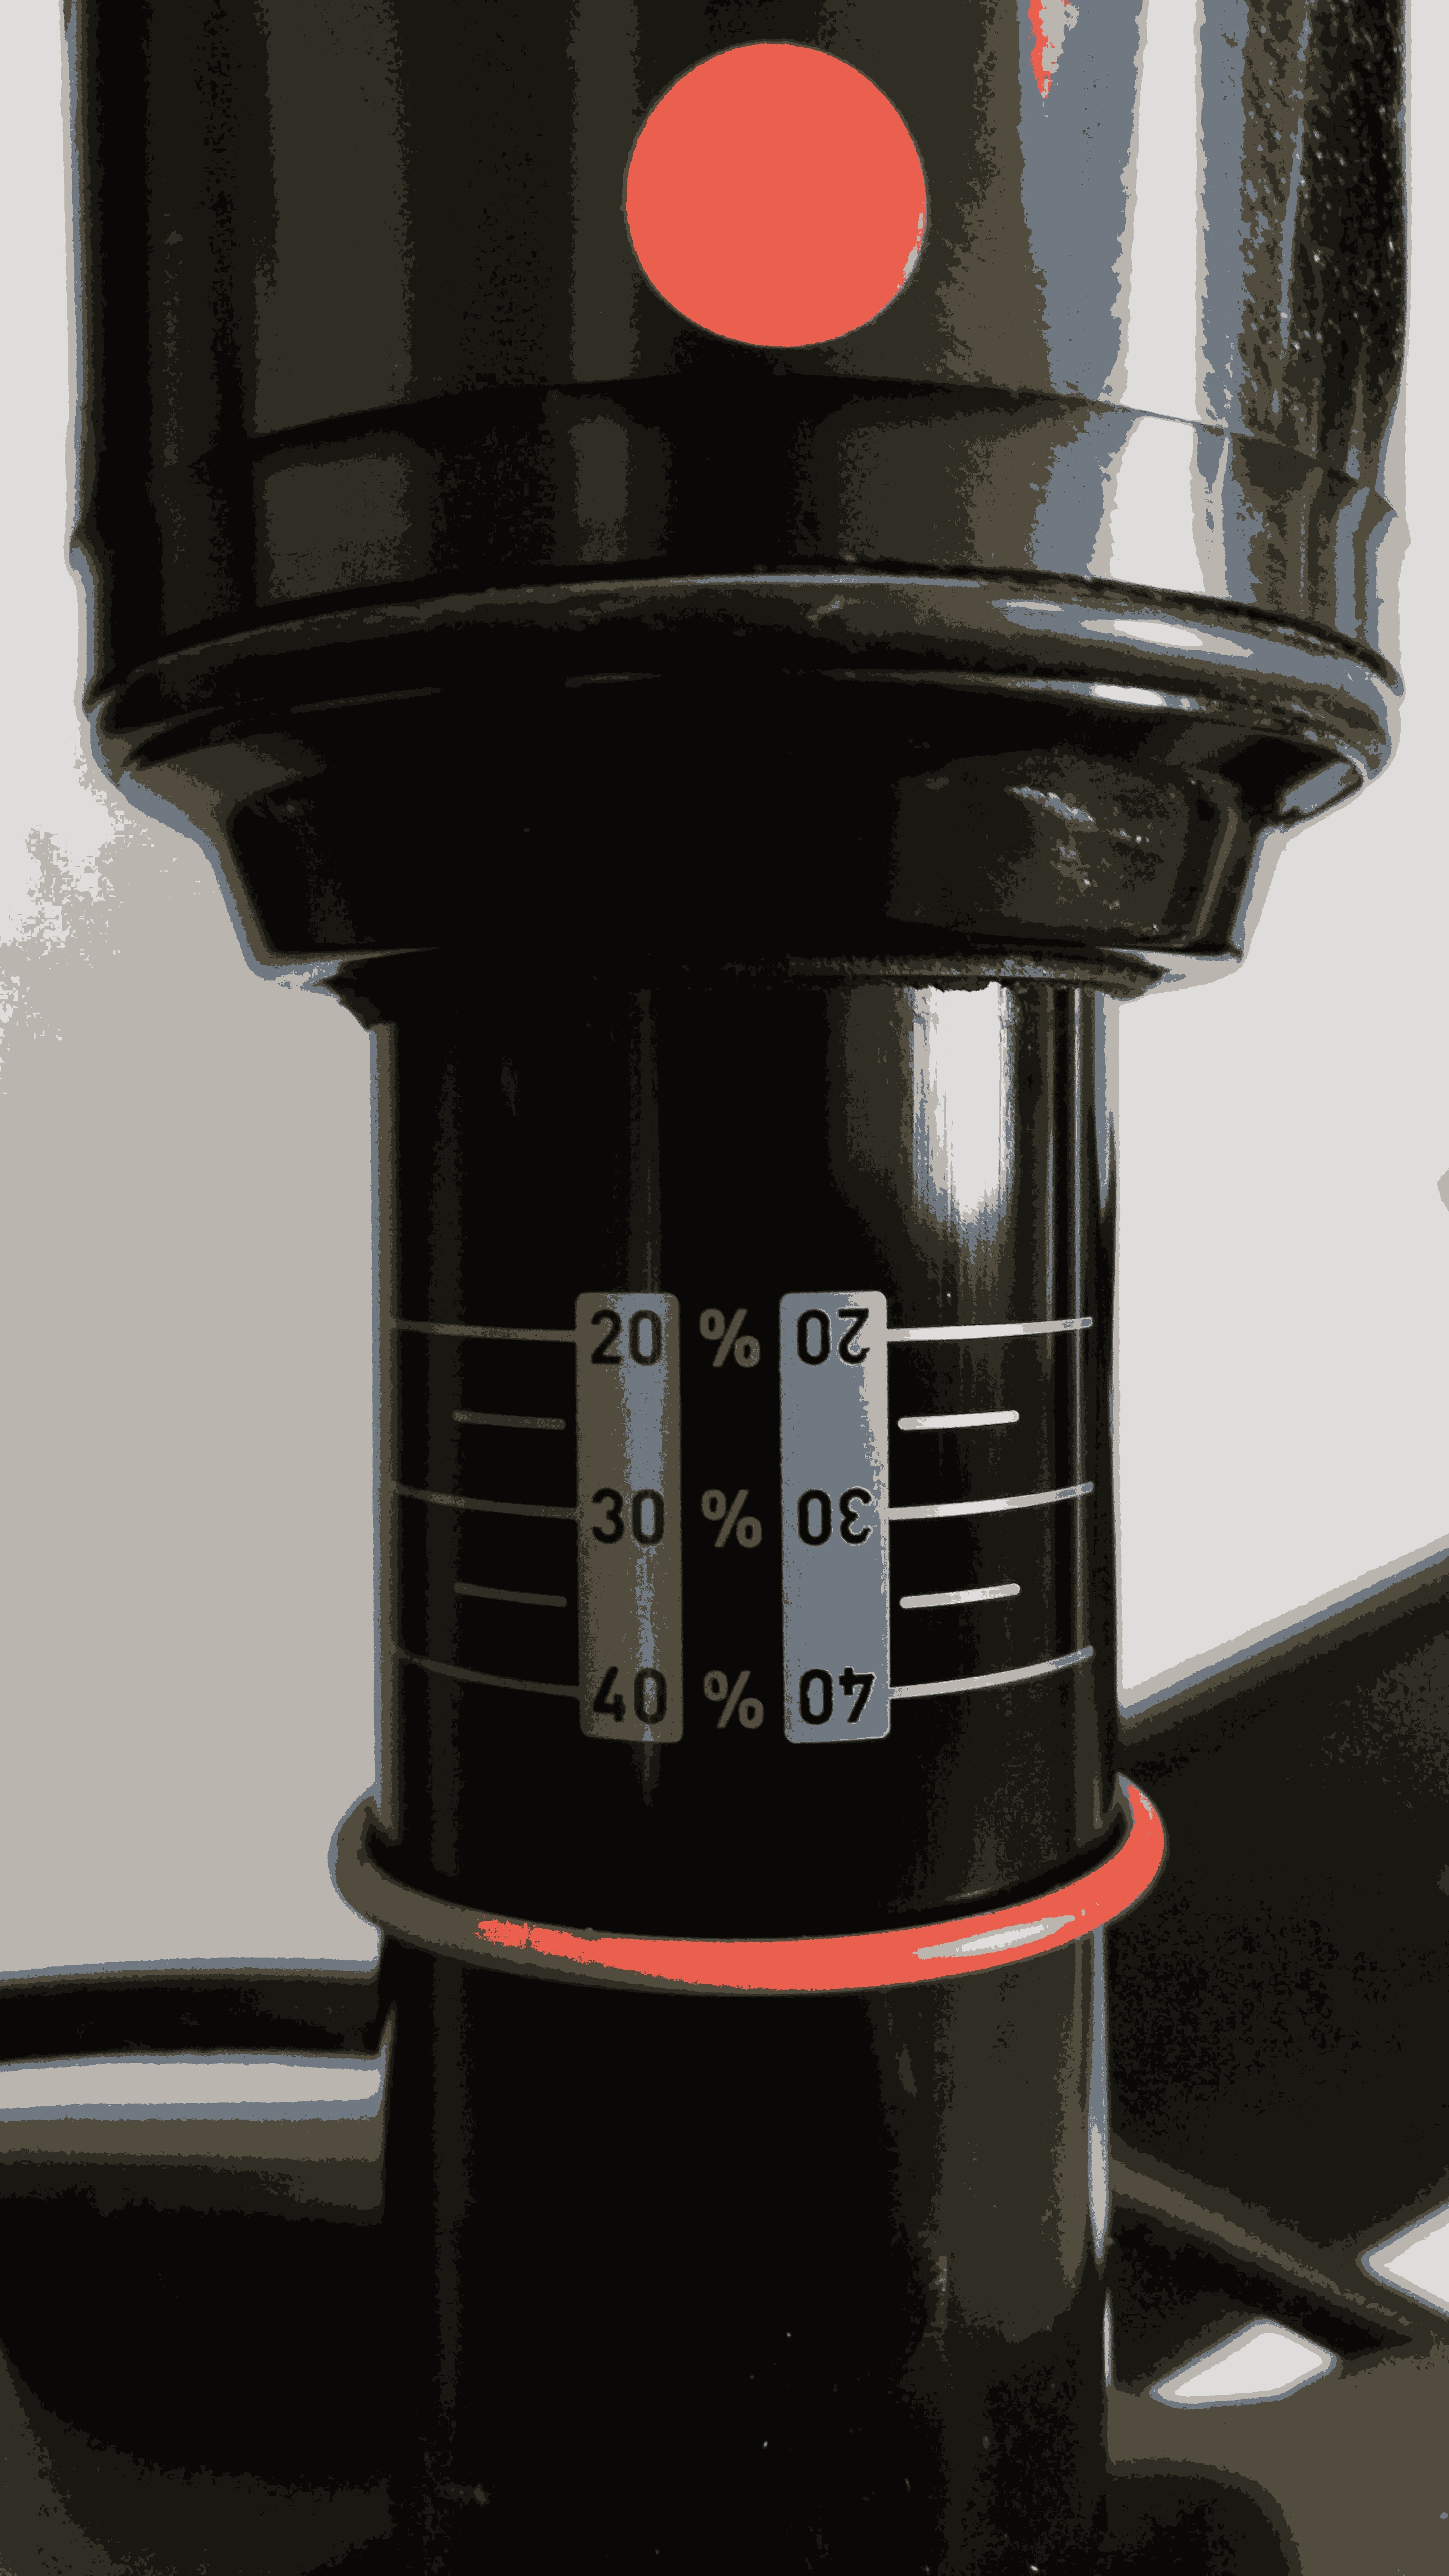
\includegraphics[scale=0.04]{../images/results/quant.jpg}
		 		\subcaption{Colour quantified image}
				\label{subfig:quantified}
			\end{subfigure}\hfill
			\begin{subfigure}[t]{0.2\textwidth}
				\centering
				
\includegraphics[scale=0.04]{../images/results/mask.jpg}
				\subcaption{Image mask}
				\label{subfig:mask}
			\end{subfigure}\hfill
			\begin{subfigure}[t]{0.2\textwidth}
				\centering
				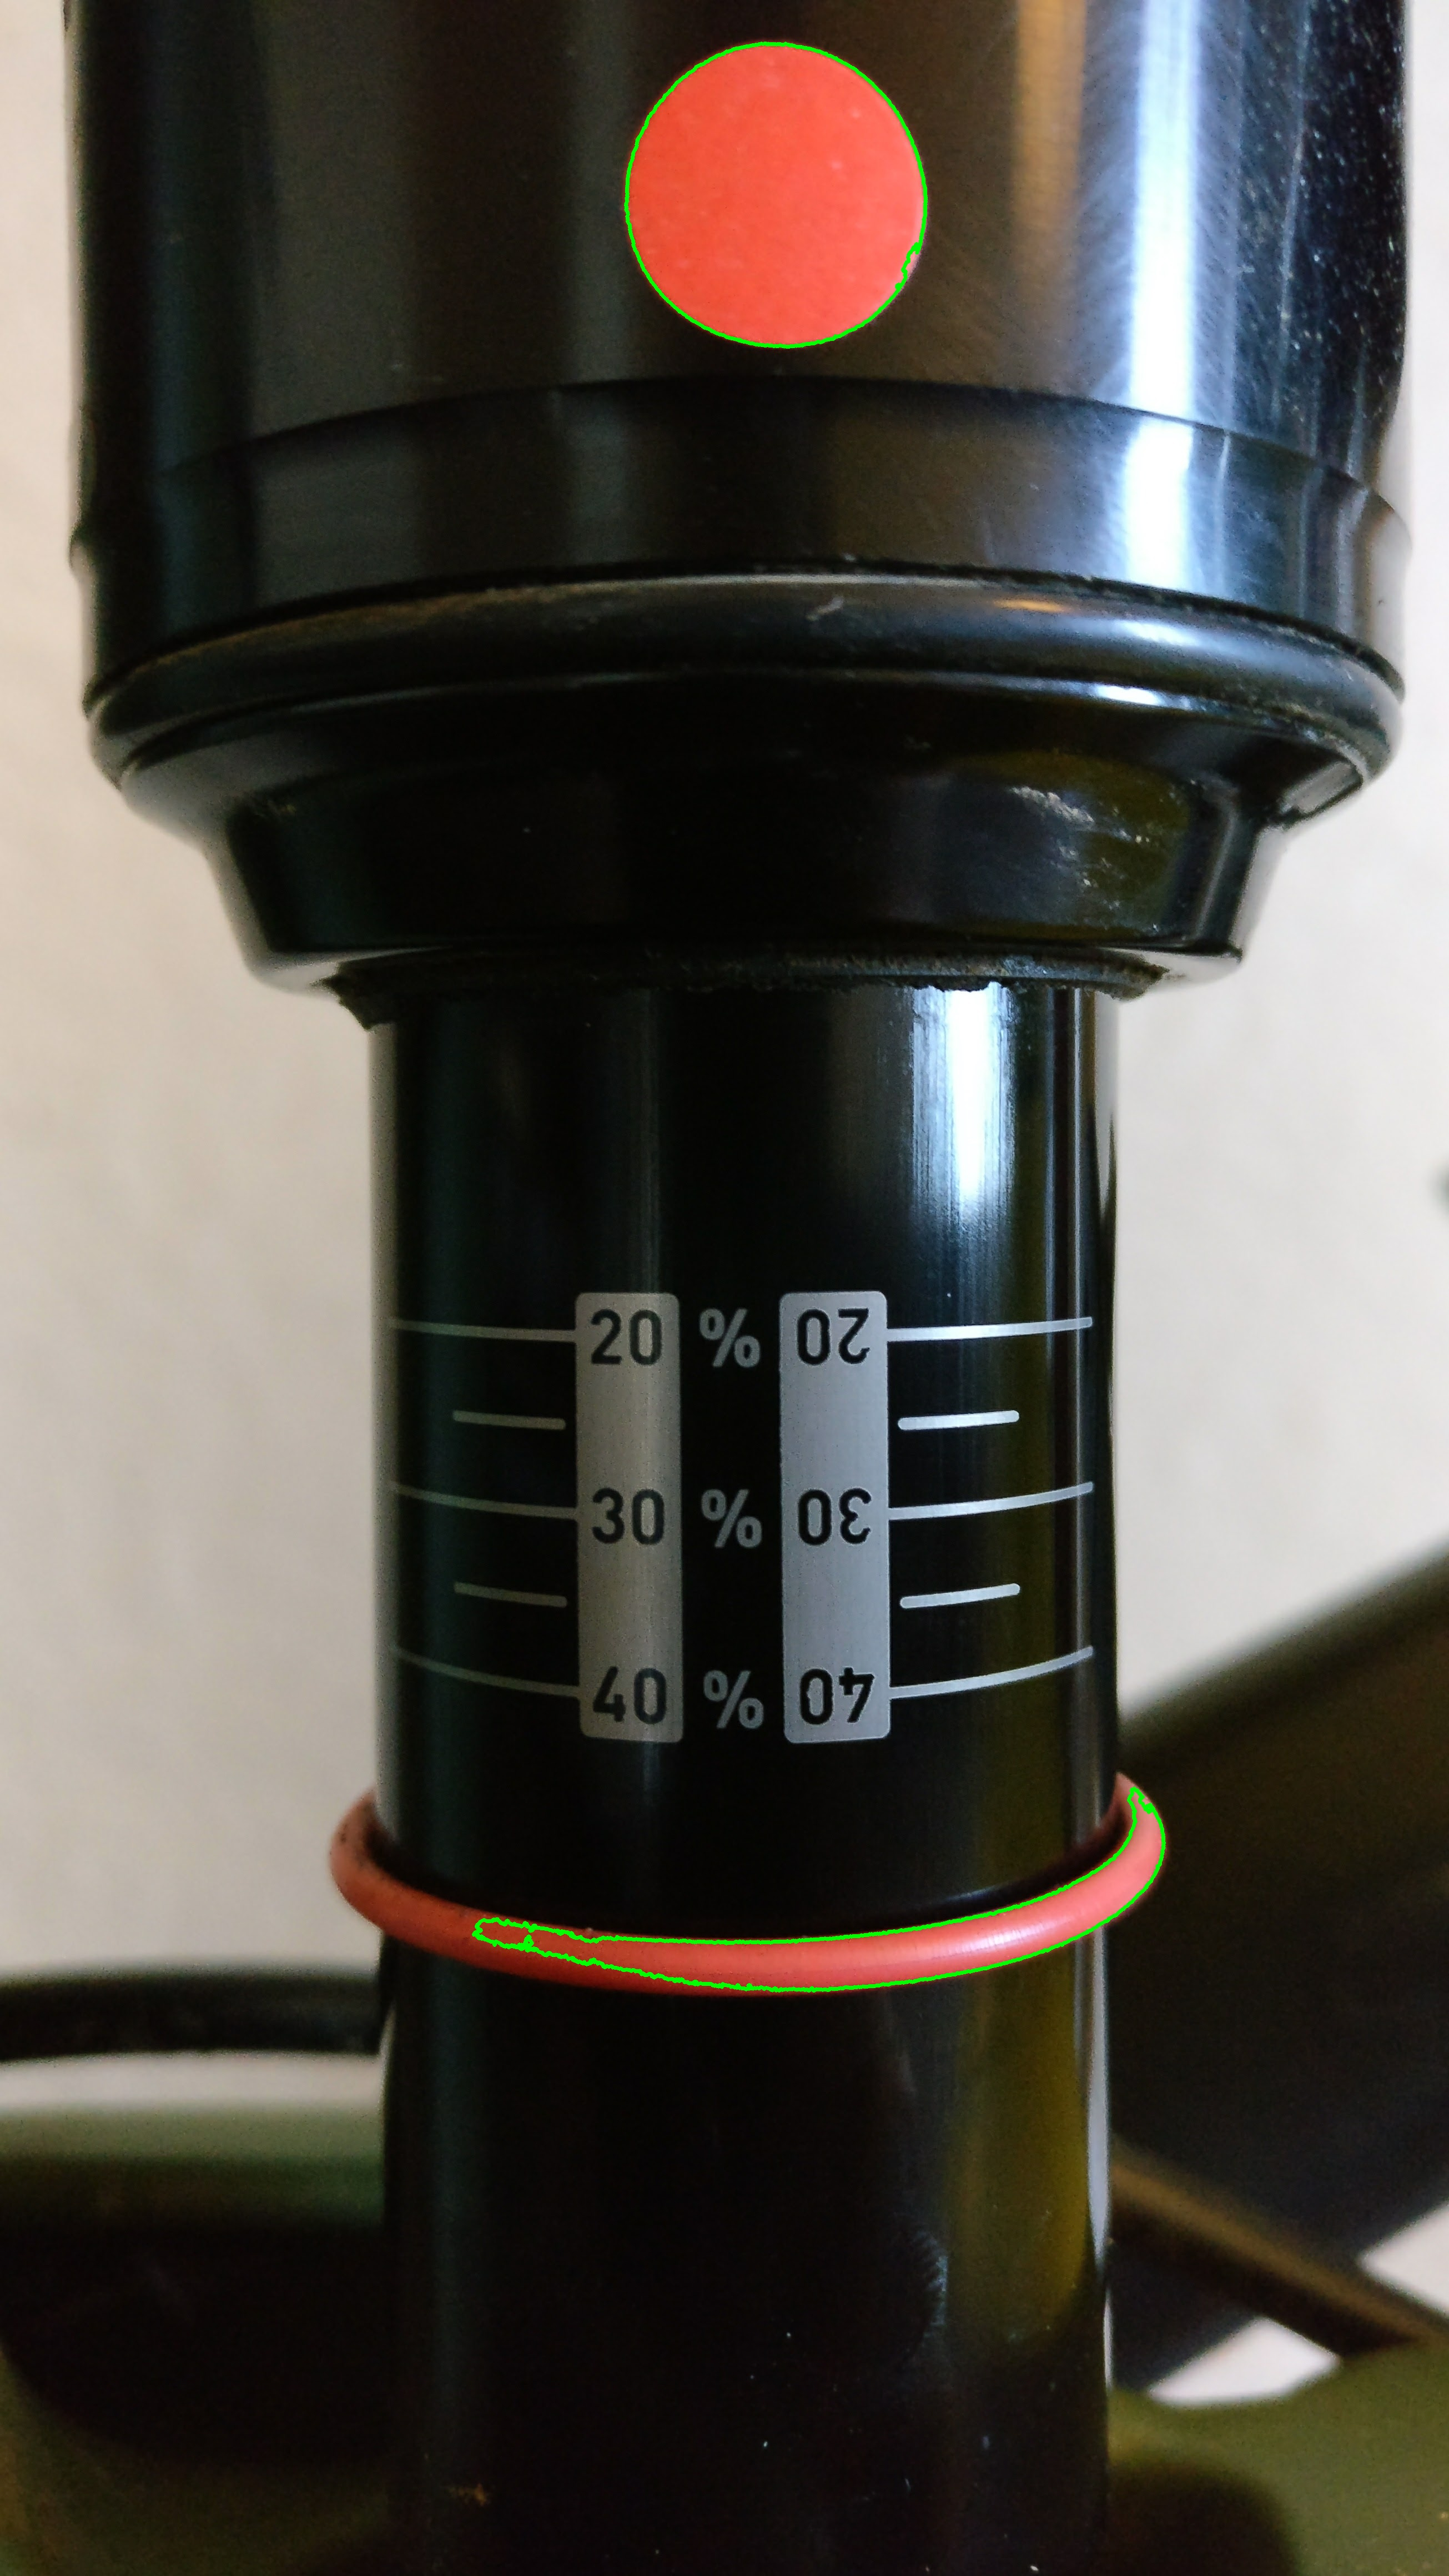
\includegraphics[scale=0.04]{../images/results/contours.jpg}
				\subcaption{Found contours from mask}
				\label{subfig:contours}
			\end{subfigure}\hfill
			\begin{subfigure}[t]{0.2\textwidth}
				\centering
				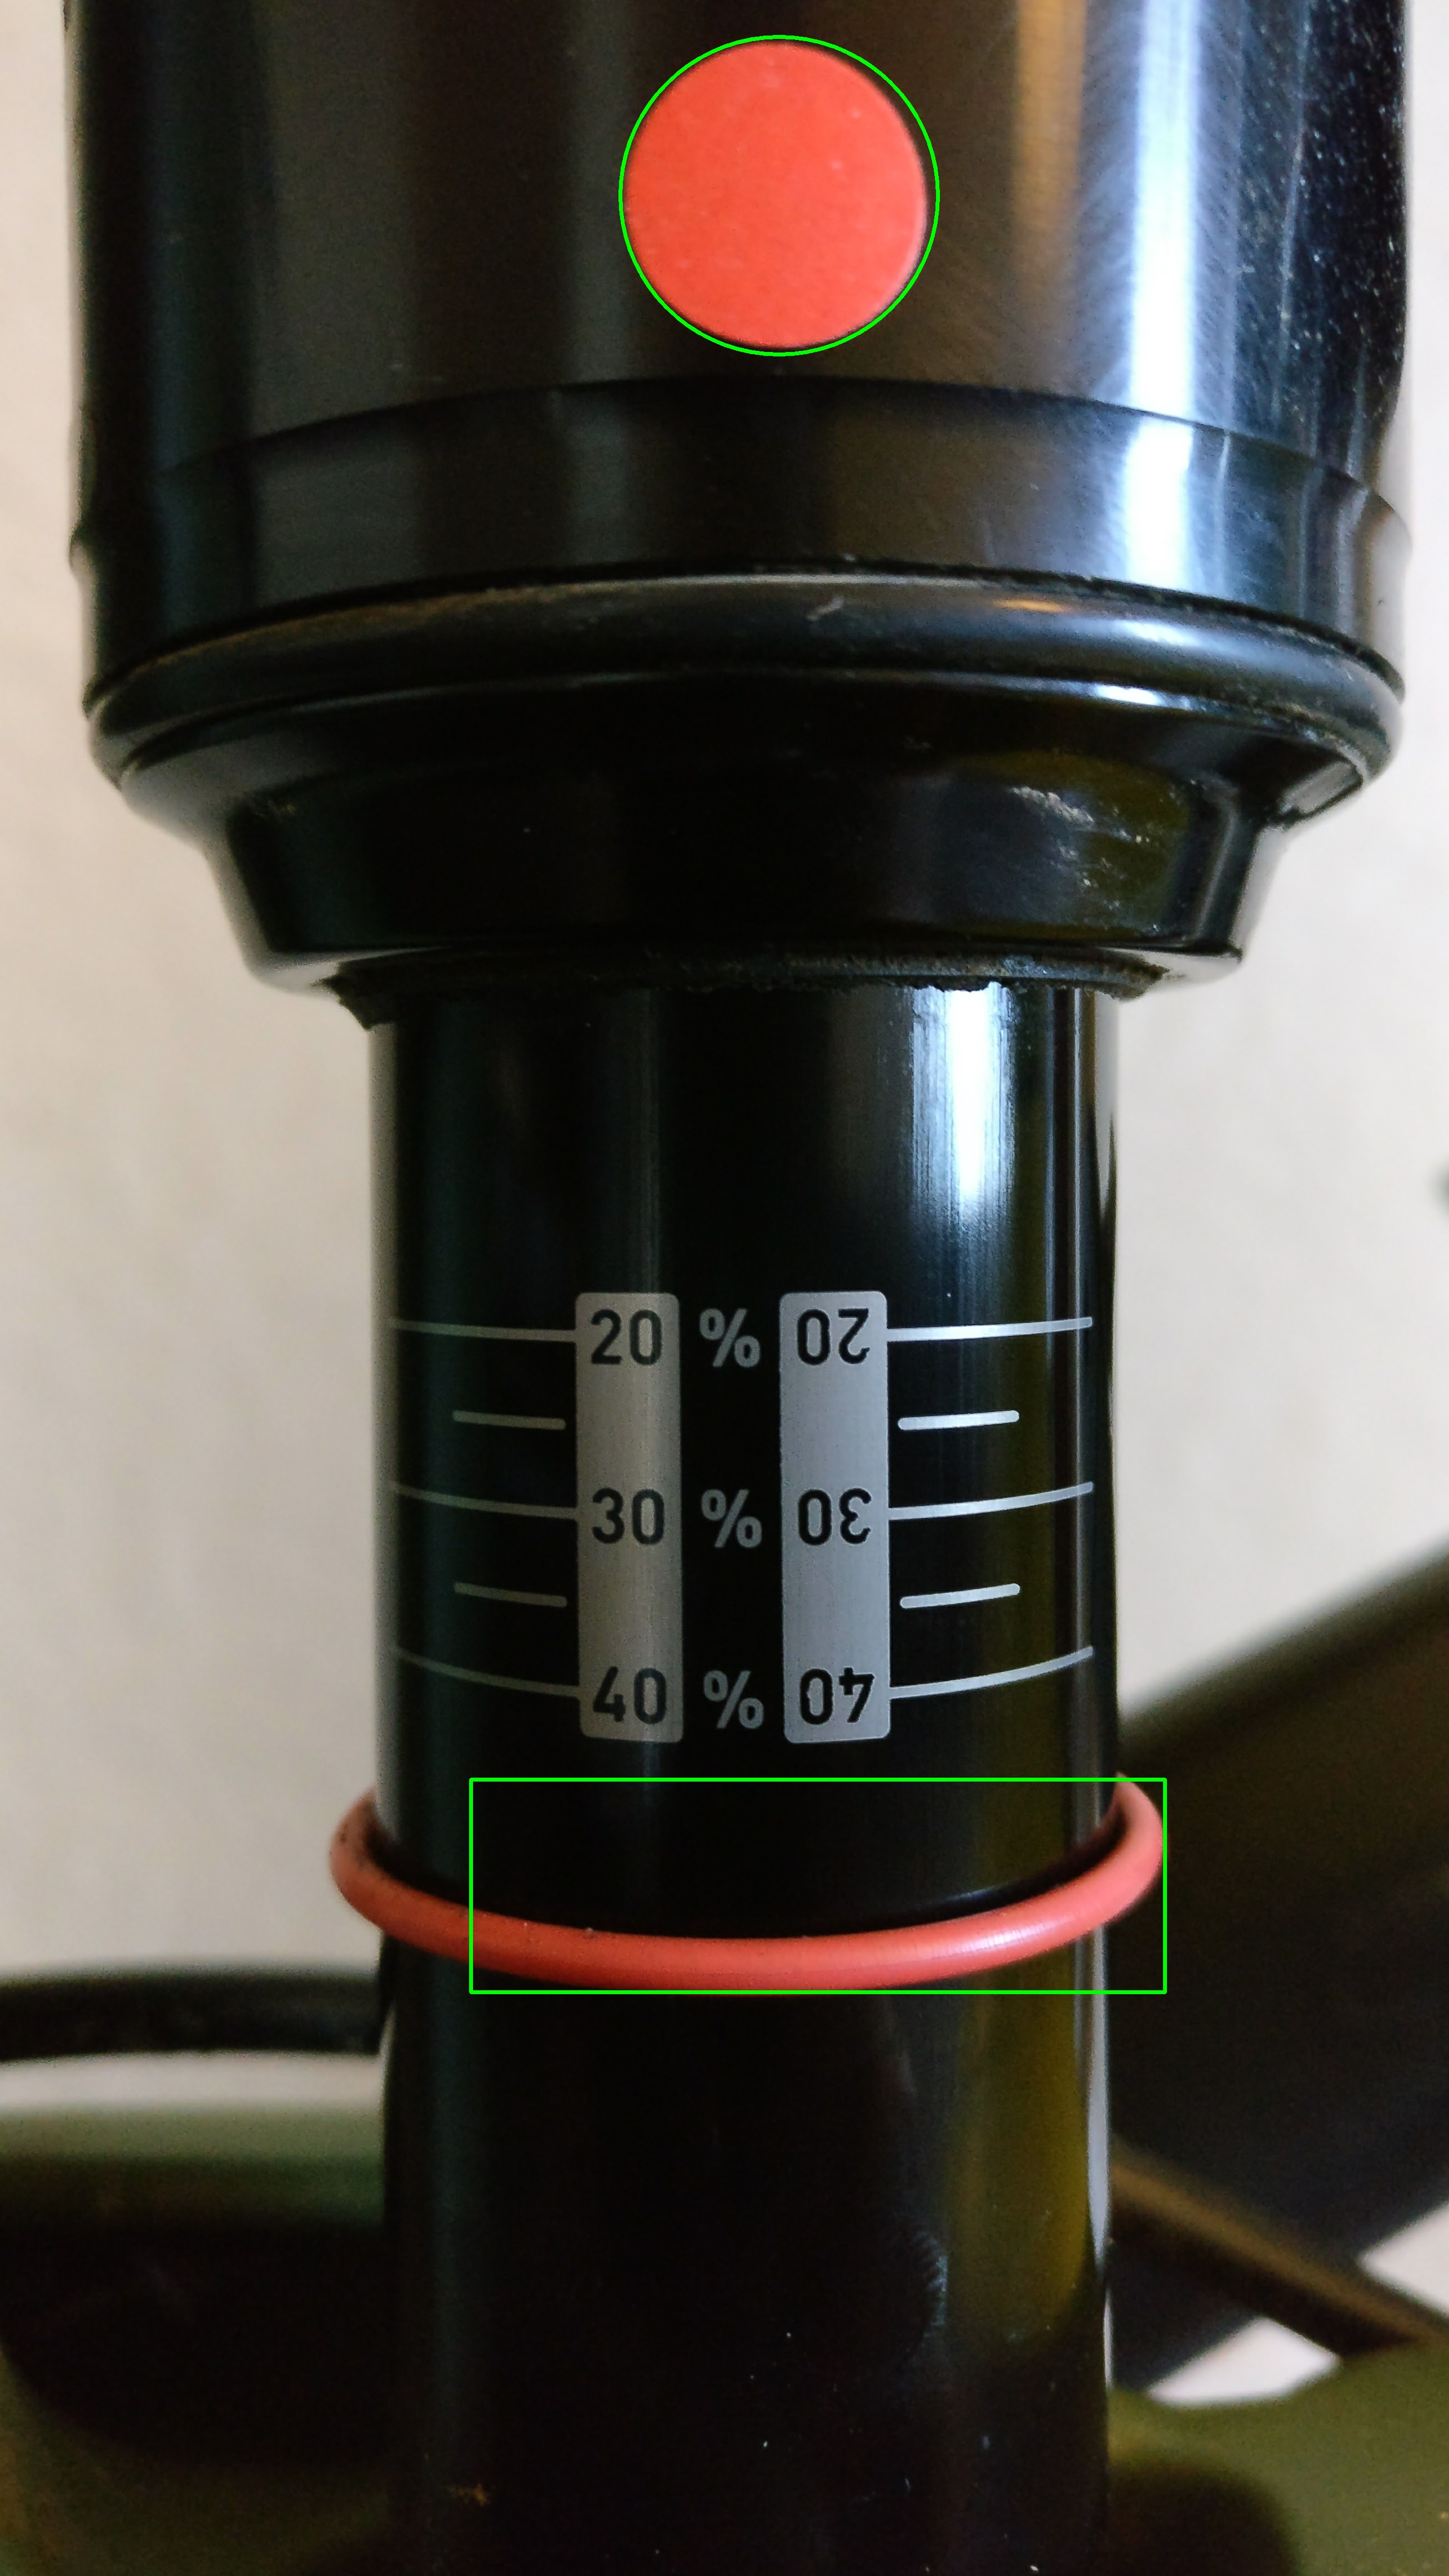
\includegraphics[scale=0.04]{../images/results/raw_refs.jpg}
				\subcaption{Bounding circle and box from contours}
				\label{subfig:boundaries}
			\end{subfigure}
			\caption{Processed images for finding reference point}
			\label{fig:ref_point_process}
		\end{figure}
		\paragraph{O-Ring}
			If a red coloured o-ring is specified then the same process to find the reference point is used. The second largest contour found will be the o-ring so a bounding box can be drawn round it from which a measurement limit can be collected. The red o-ring mask, contour, and bounding box can be seen in Figure \ref{fig:ref_point_process}.
			\\\\
			If a black o-ring is specified, an alternative process is used. Thresholding is applied to the image which highlights any shadows or highlights on the shock shaft. As these are intersected by the o-ring it is simple to select a contour which ends at the o-ring to produce a measurement limit from. This process is shown in Figure \ref{fig:fox_oring}.
		\begin{figure}[h!]
			\centering
			\begin{subfigure}[t]{0.4\textwidth}
				\centering
				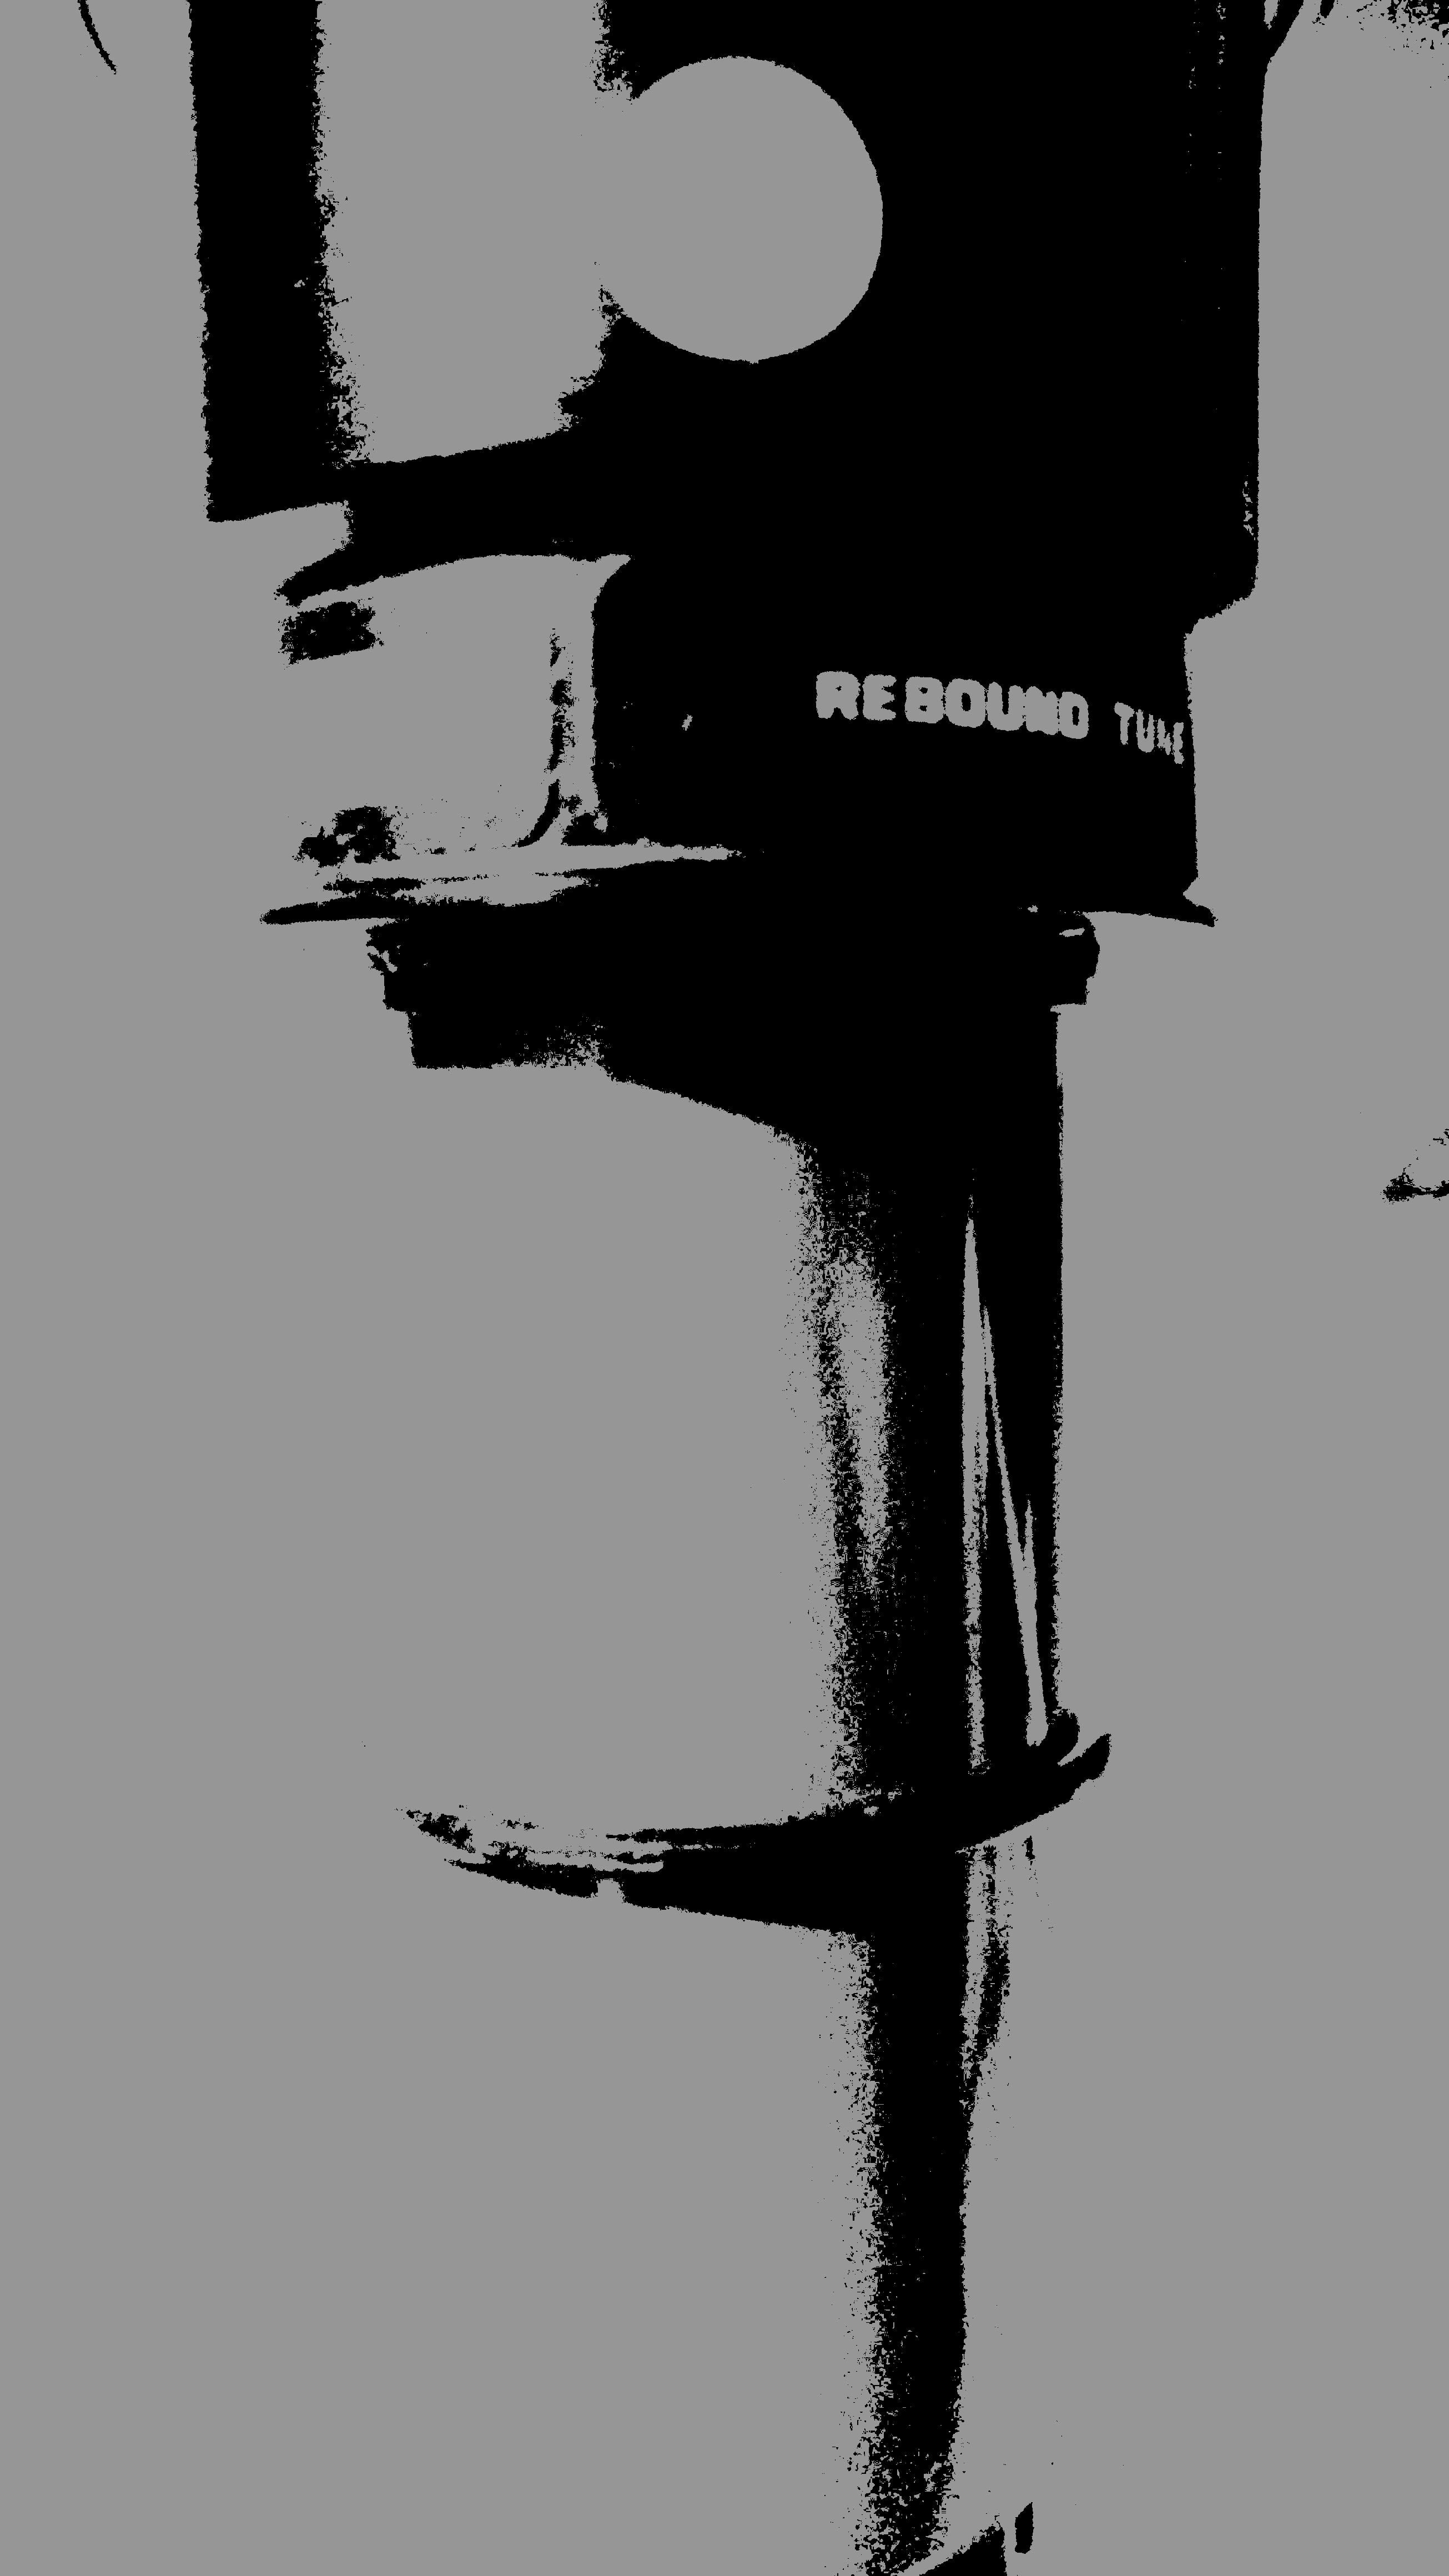
\includegraphics[scale=0.04]{../images/results/threshold.jpg}
				\subcaption{Image thresholding}
				\label{subfig:threshold}
			\end{subfigure}
			\begin{subfigure}[t]{0.4\textwidth}
				\centering
				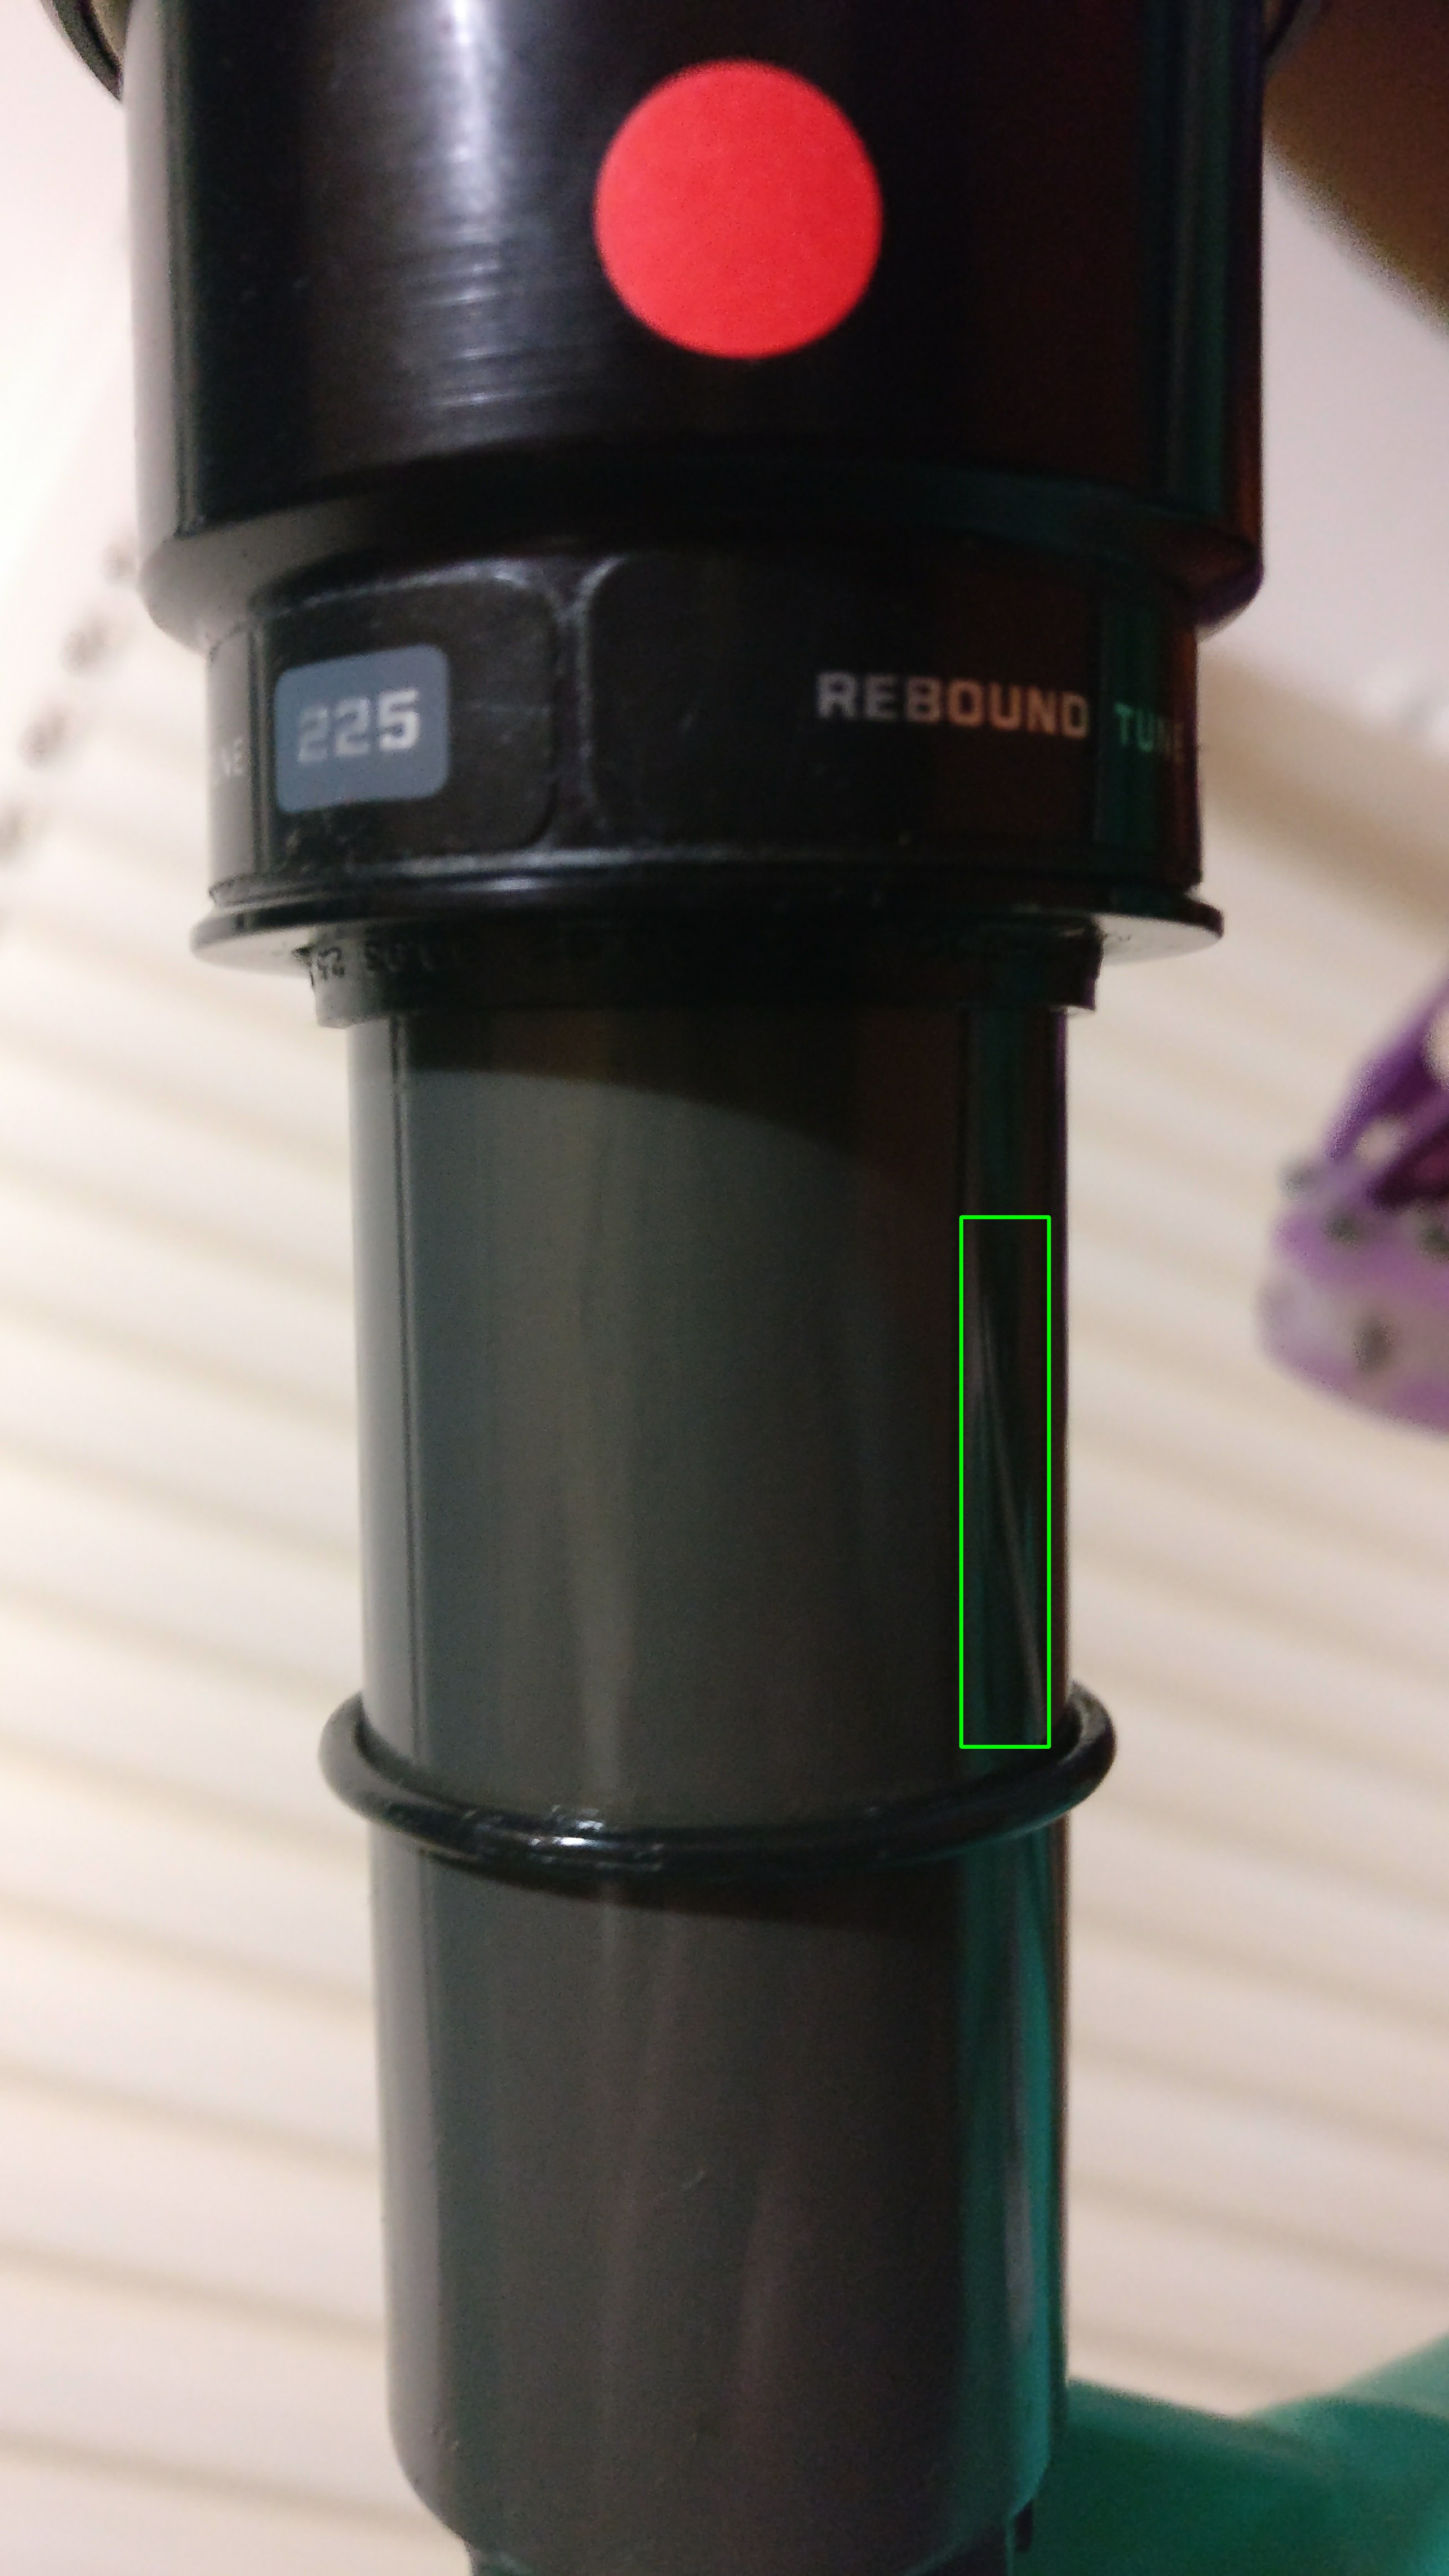
\includegraphics[scale=0.04]{../images/results/fox_oring.jpg}	
				\subcaption{O-ring indicator}
				\label{subfig:fox_oring}
			\end{subfigure}
			\caption{Locating process for black o-ring}
			\label{fig:fox_oring}
		\end{figure}
		% Edge detect
		% Lines
		% px to mm
		% Calc linear equation
		% Calc ideal sag measurement
		% Calc pressure
		\paragraph{Measurement}
			With the pixels per millimetre metric produced and the measurement limit found, the sag under the current pressure is measured. First, edge detection is carried out on the original input image to highlight the lines of the shock, this output is shown in Figure \ref{subfig:edge_detect}. Hough line transformation is then applied to locate vertical lines between the top of the shock shaft and the measurement limit. The difference in pixels between the highest and lowest points of these lines is the current sag measurement. This can be converted to millimetres using the px/mm metric.
		\begin{figure}[h!]
			\centering
			\begin{subfigure}[t]{0.4\textwidth}
				\centering
				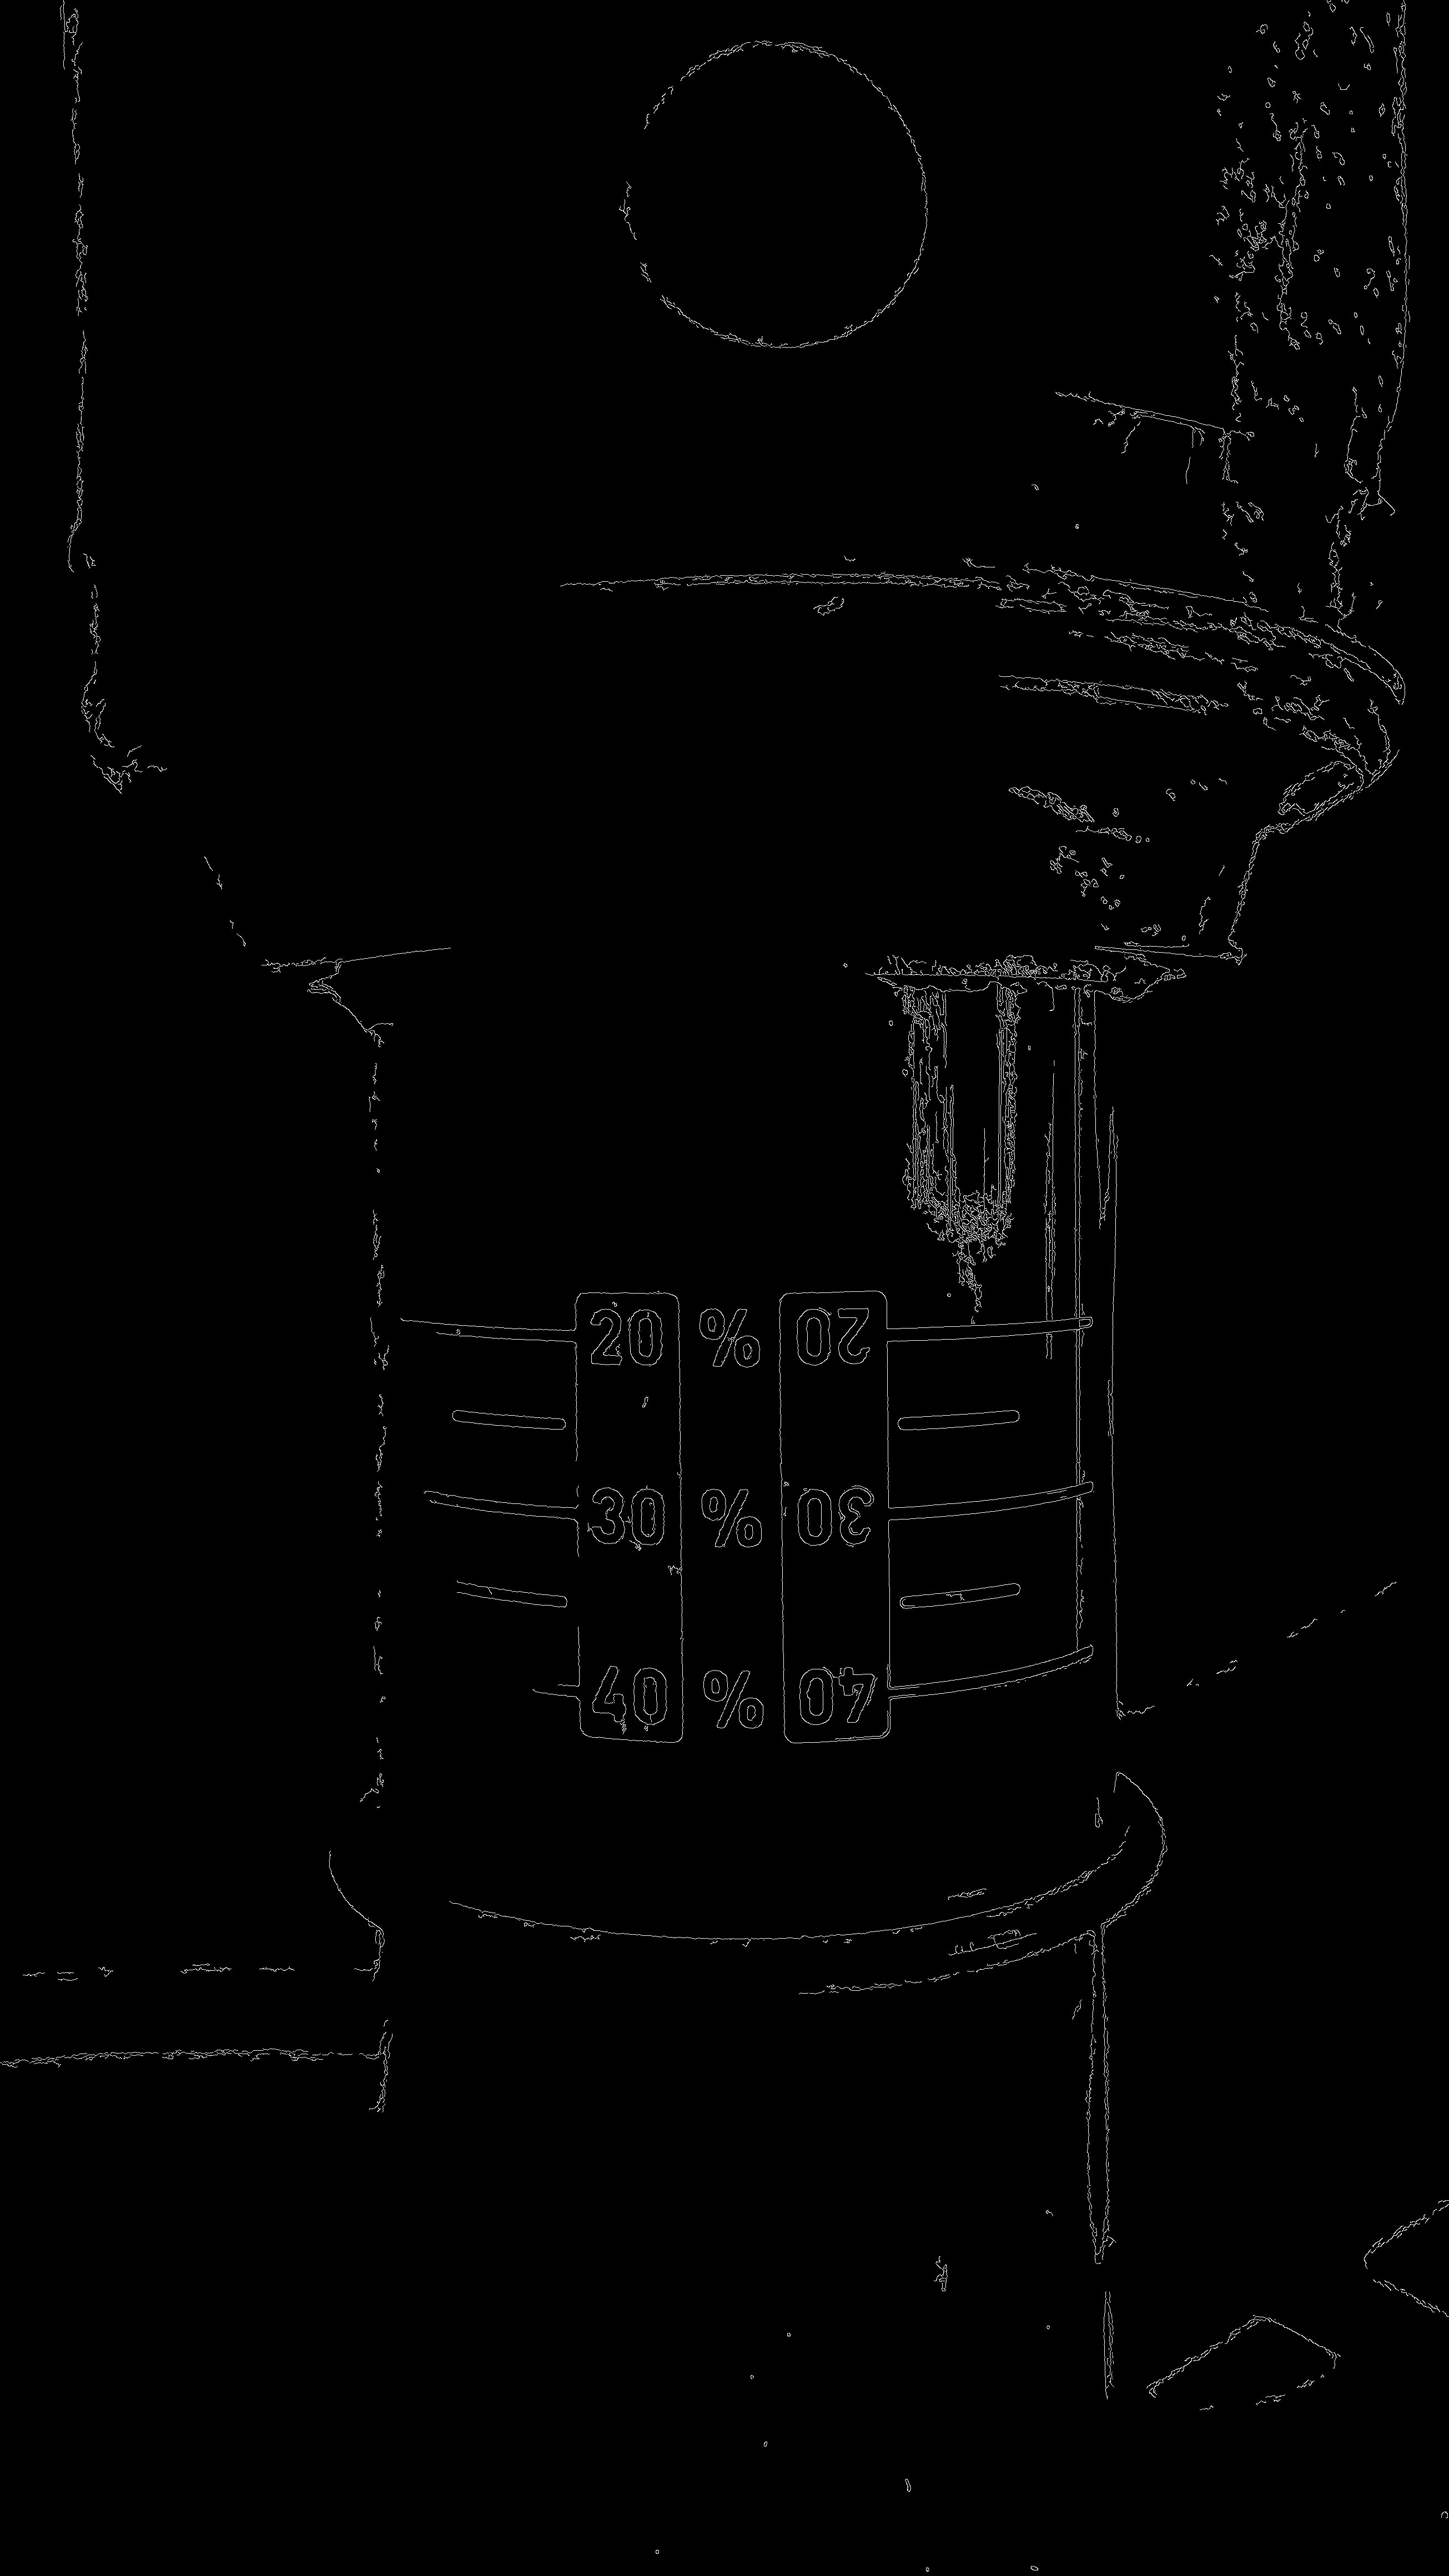
\includegraphics[scale=0.04]{../images/results/edged.jpg}
				\caption{Edge detected image}
				\label{subfig:edge_detect}
			\end{subfigure}
			\begin{subfigure}[t]{0.4\textwidth}
				\centering
				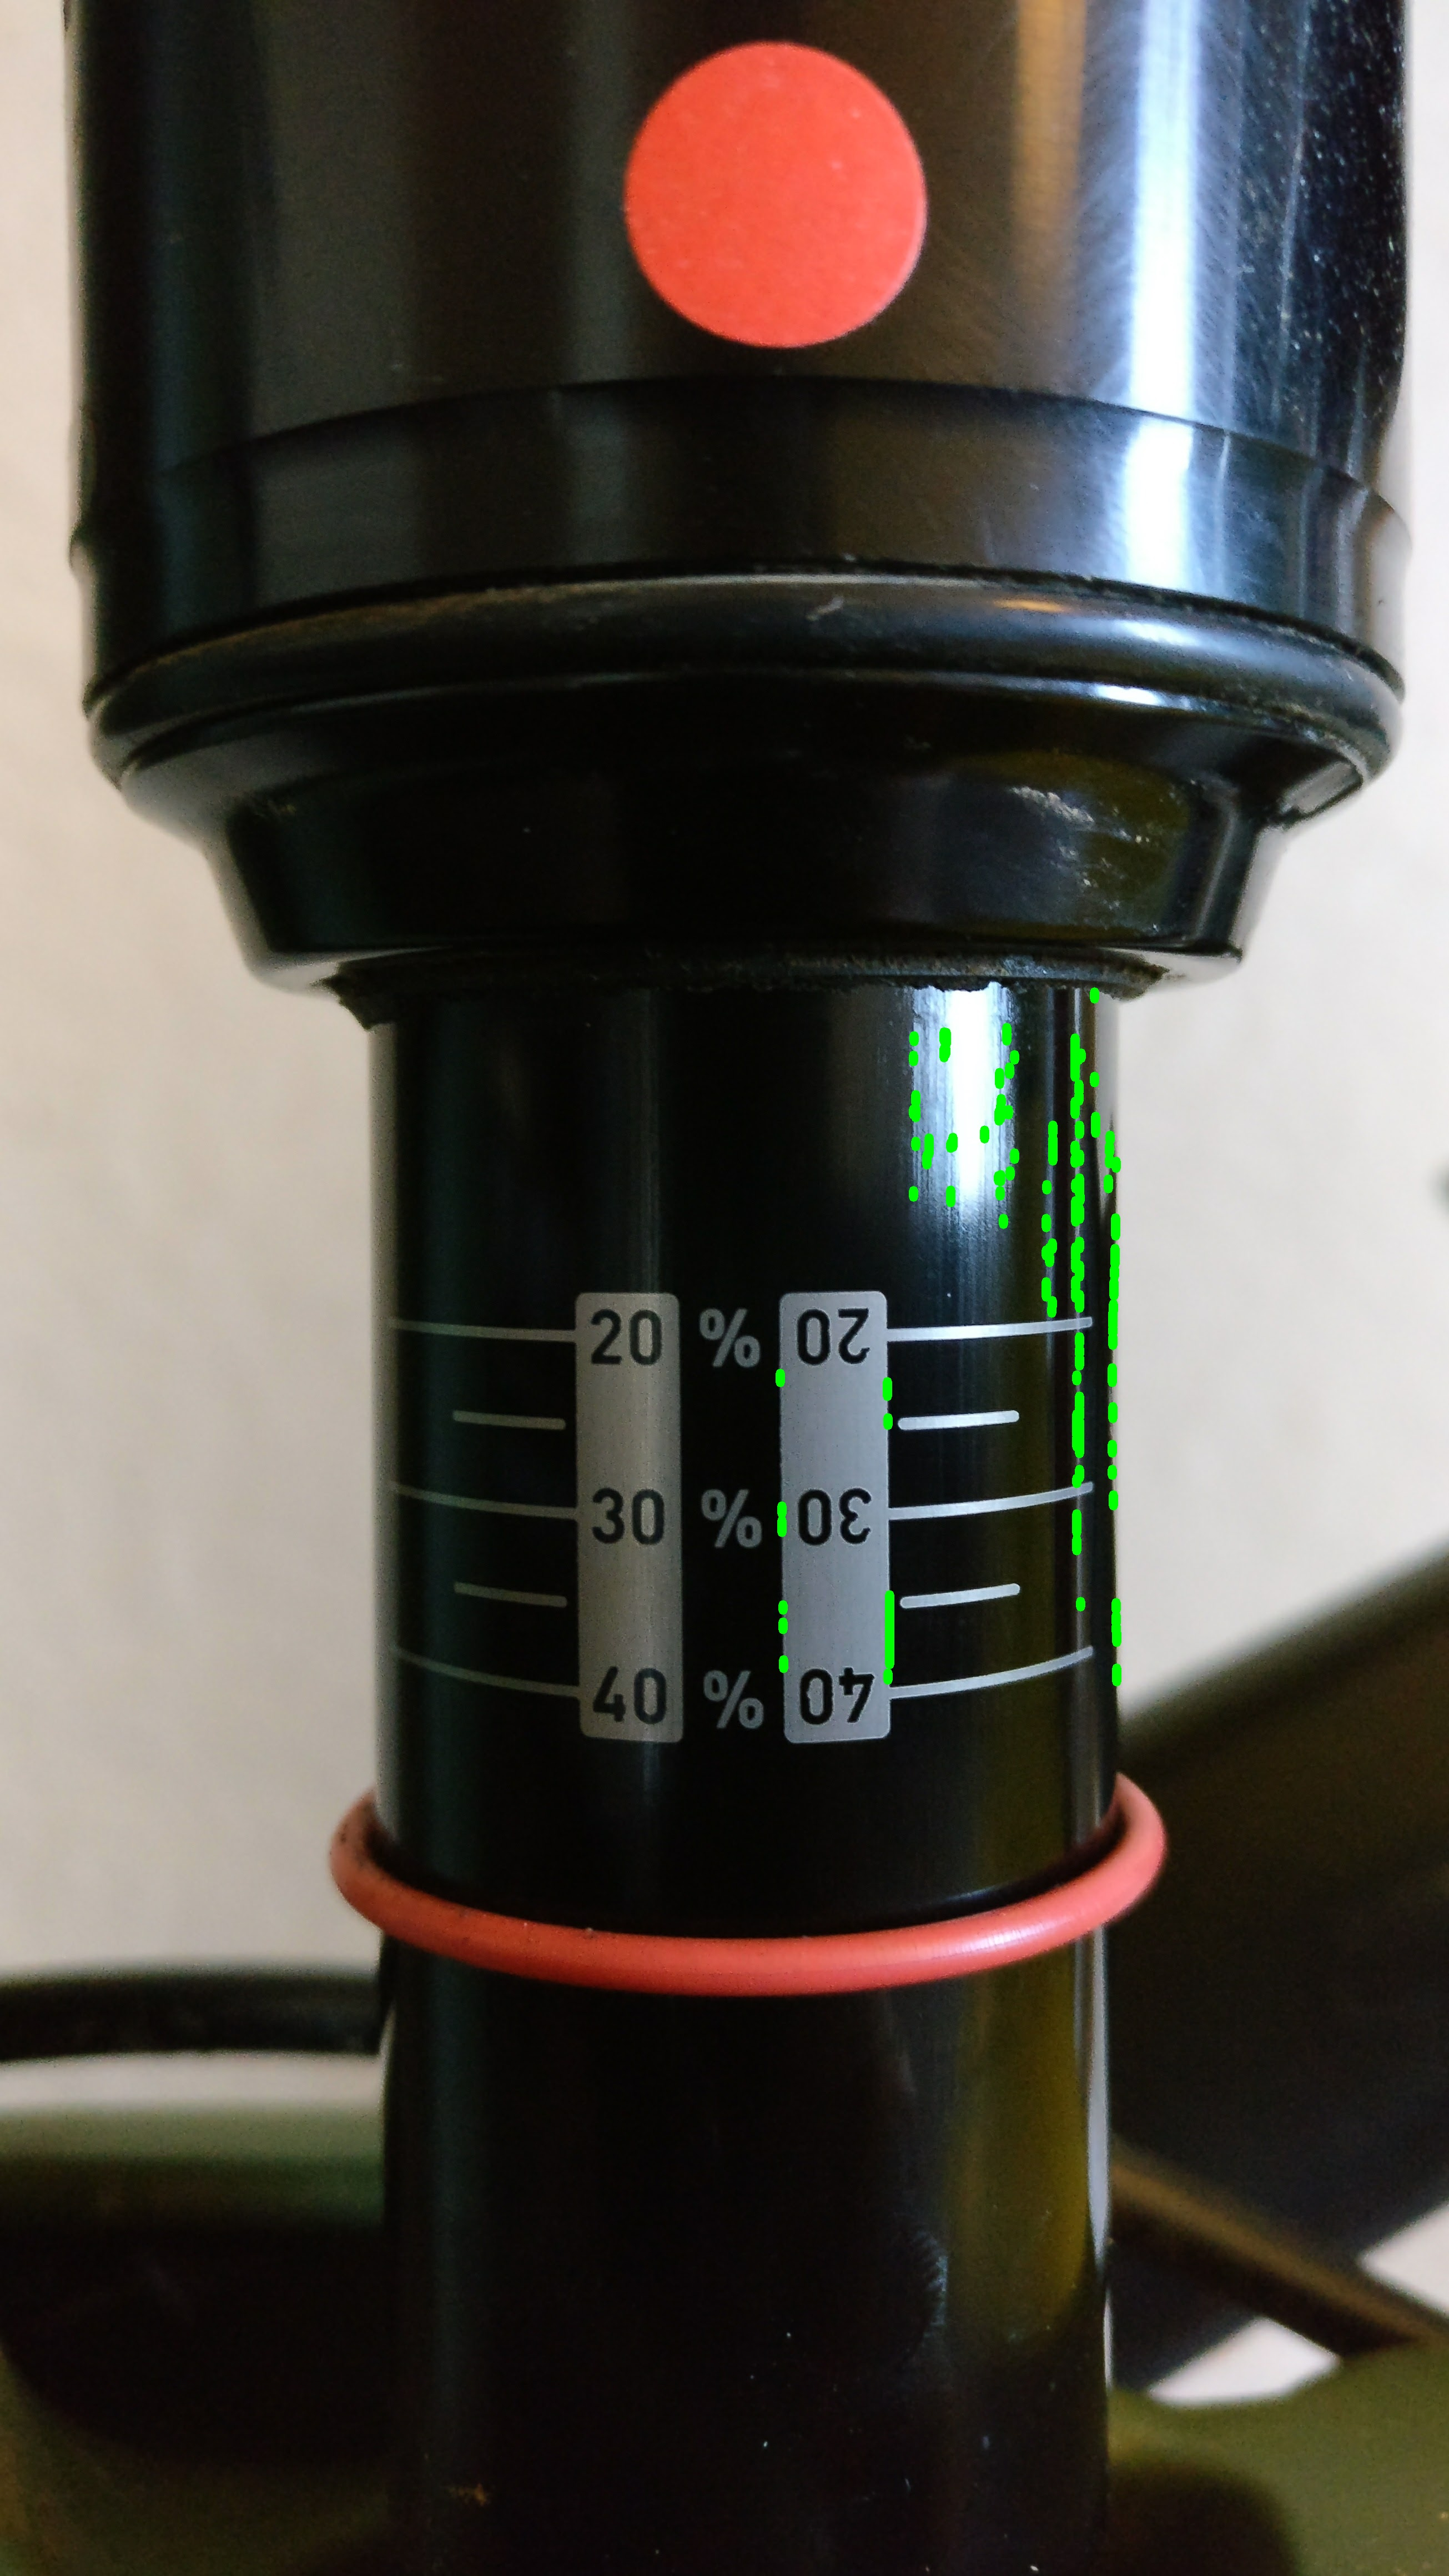
\includegraphics[scale=0.085,
								trim={40cm 35cm 10cm 50cm},
								clip]{../images/results/raw_lines.jpg}
				\caption{Vertical lines in measurement area}
				\label{subfig:lines}
			\end{subfigure}
		\end{figure}
		\paragraph{Equation}
			Once the measurements for the shock pressurised to 100psi and 150psi are produced, they can then be utilised to create a linear equation. This is carried out using Python's Scipy package and its linregress method which accepts two arrays of data and returns the slope and intercept of the linear equation. The equation is visually described in Figure \ref{fig:equation_plot}; it should be noted that this plot is only produced virtually and never output to the user.
			\begin{figure}[h!]
				\centering
				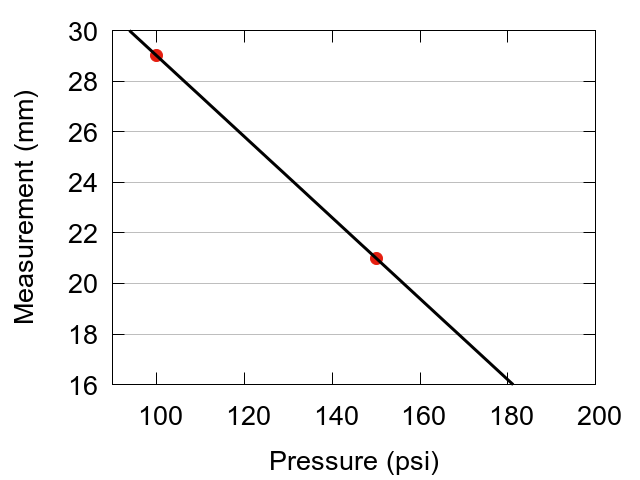
\includegraphics[scale=0.4]{../images/results/scatter_key.png}
				\caption{Example of linear equation plot}
				\label{fig:equation_plot}
			\end{figure}
		\paragraph{Produce Setting}
\clearpage
\subsection{Critical Evaluation}
	\subsubsection{Validation}
	\subsubsection{Reliability and Accuracy}
		\begin{table}[h!]
			\centering
			\caption{Table of uncertainty calculation results}
			\label{tab:uncertainty}
		\begin{tabular}{|l|r|r|r|r|}
			\hline
			\multirow{12}{7em}{\bfseries Measurements}&\multicolumn{2}{|l|}{\bfseries Rockshox}&\multicolumn{2}{|l|}{\bfseries Fox}\\
			\cline{2-5}
			&\bfseries 25\%&\bfseries 30\%&\bfseries 25\%&\bfseries 30\%\\
			\hline
			&175.02&160.97&133.31&120.54\\
			&174.84&160.52&133.28&120.47\\
			&174.95&160.41&133.42&120.48\\
			&174.83&160.65&133.42&120.46\\
			&174.94&160.75&133.29&120.53\\
			&174.86&160.50&133.38&120.51\\
			&175.63&160.48&133.35&120.50\\
			&174.78&160.77&133.36&120.46\\
			&175.29&160.57&133.36&120.46\\
			&174.84&160.74&133.42&120.50\\
			\hline
			\bfseries Average&175.00&160.64&133.36&120.49\\
			\bfseries Standard Deviation&0.27&0.17&0.05&0.03\\
			\bfseries Uncertainty&175 $\pm$ 0.27&160.64 $\pm$ 0.17&133.36 $\pm$ 0.05&120.49 $\pm$ 0.03\\
			\hline
		\end{tabular}
		\end{table}
	\subsubsection{Comparison to Alternatives}
	\subsubsection{Professional Opinion}